% Professional M.Tech Thesis Template
% Compile with: xelatex main.tex && bibtex main && xelatex main.tex && xelatex main.tex
\documentclass[11pt, a4paper, twoside, openany]{book}

% --- XeLaTeX Font Setup ---
\usepackage{fontspec}
\usepackage{unicode-math}

\setmainfont{AGaramondPro}[
  Path           = fonts/,
  Extension      = .otf,
  UprightFont    = *-Regular,
  BoldFont       = *-Bold,
  ItalicFont     = *-Italic,
  BoldItalicFont = *-BoldItalic
]
\setsansfont{AGaramondPro}[
  Path           = fonts/,
  Extension      = .otf,
  UprightFont    = *-Regular,
  BoldFont       = *-Bold,
  ItalicFont     = *-Italic,
  BoldItalicFont = *-BoldItalic
]
\setmonofont{AptosMono}[
  Path           = fonts/,
  Extension      = .otf,
  UprightFont    = *-Regular,
  BoldFont       = *-Bold,
  ItalicFont     = *-Italic,
  BoldItalicFont = *-BoldItalic,
  Scale          = MatchLowercase
]
\setmathfont{TeX Gyre Termes Math}

% --- Page Layout ---
\usepackage[
  a4paper,
  inner=3cm,
  outer=2.5cm,
  top=2.0cm,
  bottom=2.0cm
]{geometry}

% --- Typography ---
\usepackage{microtype}
\usepackage{setspace}
\setstretch{1.2}

% --- Packages ---
\usepackage{graphicx}
\graphicspath{{figures/}}
\usepackage{eso-pic}
\usepackage[hidelinks]{hyperref}
\usepackage{titlesec}
\usepackage{tocloft}
\usepackage{fancyhdr}
\usepackage{enumitem}
\setlist{noitemsep, topsep=0pt, partopsep=0pt, parsep=0pt}
\usepackage{caption}
\usepackage{subcaption}
\usepackage{booktabs}
\usepackage{multirow}
\usepackage{array}
\usepackage{longtable}
\usepackage{float}
\usepackage{amsmath}
% \usepackage{amssymb}
\usepackage{algorithmic}
\usepackage{algorithm}
\usepackage{xcolor}
\usepackage{tabularx}
\usepackage{tikz}
\usetikzlibrary{shapes.geometric, arrows.meta, positioning}
\usepackage{pgfplots}
\pgfplotsset{compat=1.18}
\usepackage{pdfpages}

% --- Caption Styling ---
\captionsetup{
  font=small,
  labelfont=bf
}

% --- Header/Footer ---
\pagestyle{fancy}
\fancyhf{}
\fancyhead[LE]{\textsf{\small\textsc{\leftmark}}}
\fancyhead[RO]{\textsf{\small\textsc{\rightmark}}}
\fancyhead[RE,LO]{\thepage}
\renewcommand{\headrulewidth}{0.4pt}

% Empty page style
\fancypagestyle{empty}{%
  \fancyhf{}
  \renewcommand{\headrulewidth}{0pt}
  \renewcommand{\footrulewidth}{0pt}
}

% Plain page style (chapter opening pages)
\fancypagestyle{plain}{%
  \fancyhf{}
  \fancyfoot[C]{\thepage}
  \renewcommand{\headrulewidth}{0pt}
  \renewcommand{\footrulewidth}{0pt}
}

% Clean blank pages between chapters
\makeatletter
\def\cleardoublepage{\clearpage\if@twoside \ifodd\c@page\else
    \thispagestyle{empty}
    \hbox{}\newpage\fi\fi}
\makeatother

% --- Chapter Title Formatting ---
\titleformat{\chapter}[display]
  {\normalfont\sffamily\bfseries}
  {\large\chaptername\ \thechapter}
  {10pt}
  {\huge}
  [\vspace{2pt}\titlerule]

\titlespacing*{\chapter}
  {0pt}{10pt}{20pt}

% --- Section Formatting ---
\titleformat{\section}
  {\normalfont\sffamily\Large\bfseries}
  {\thesection}{1em}{}

\titleformat{\subsection}
  {\normalfont\sffamily\large\bfseries}
  {\thesubsection}{1em}{}

\titleformat{\subsubsection}
  {\normalfont\sffamily\normalsize\bfseries}
  {\thesubsubsection}{1em}{}

% --- Table of Contents ---
\renewcommand{\cftchapdotsep}{\cftdotsep}
\renewcommand{\cftchapleader}{\cftdotfill{\cftchapdotsep}}

% --- Document ---
\begin{document}

\frontmatter

% --- Title Page ---
\fancypagestyle{titlepagestyle}{%
  \fancyhf{}
  \renewcommand{\headrulewidth}{0pt}
  \renewcommand{\footrulewidth}{0.4pt}
  \fancyfoot[C]{\small \copyright\ \the\year\ Ayush Jha. All rights reserved.\\
  This work is the property of IIT (ISM) Dhanbad.\\
  No part may be reproduced without permission of the copyright holders.}
}

\begin{titlepage}
\thispagestyle{titlepagestyle}
\begin{center}

\vspace*{0.5cm}

{\huge\sffamily\bfseries Diabetic Retinopathy Classification\\[6pt] using Deep Learning and\\[6pt] Ordinal Regression \par}
\vspace{1.5cm}

{\Large\scshape A thesis submitted for the degree of\\[4pt]
Master of Technology \par}
\vspace{1.2cm}

{\Large by\\[6pt]
\textbf{Ayush Jha}\par}
\vspace{0.5cm}


\includegraphics[width=0.25\textwidth]{IIT_(ISM)_Dhanbad_Logo.eps}
\vspace{1cm}

{\large Under the supervision of\\[4pt]
\textbf{Prof. Neeru Bala}\par}
\vspace{1cm}

{\large\begin{spacing}{1.1}
Department of Mathematics and Computing\\
Indian Institute of Technology (Indian School of Mines)\\
Dhanbad
\end{spacing}\par}
\vspace{1cm}

{\large May 2026}

\end{center}
\end{titlepage}

% Included Documents
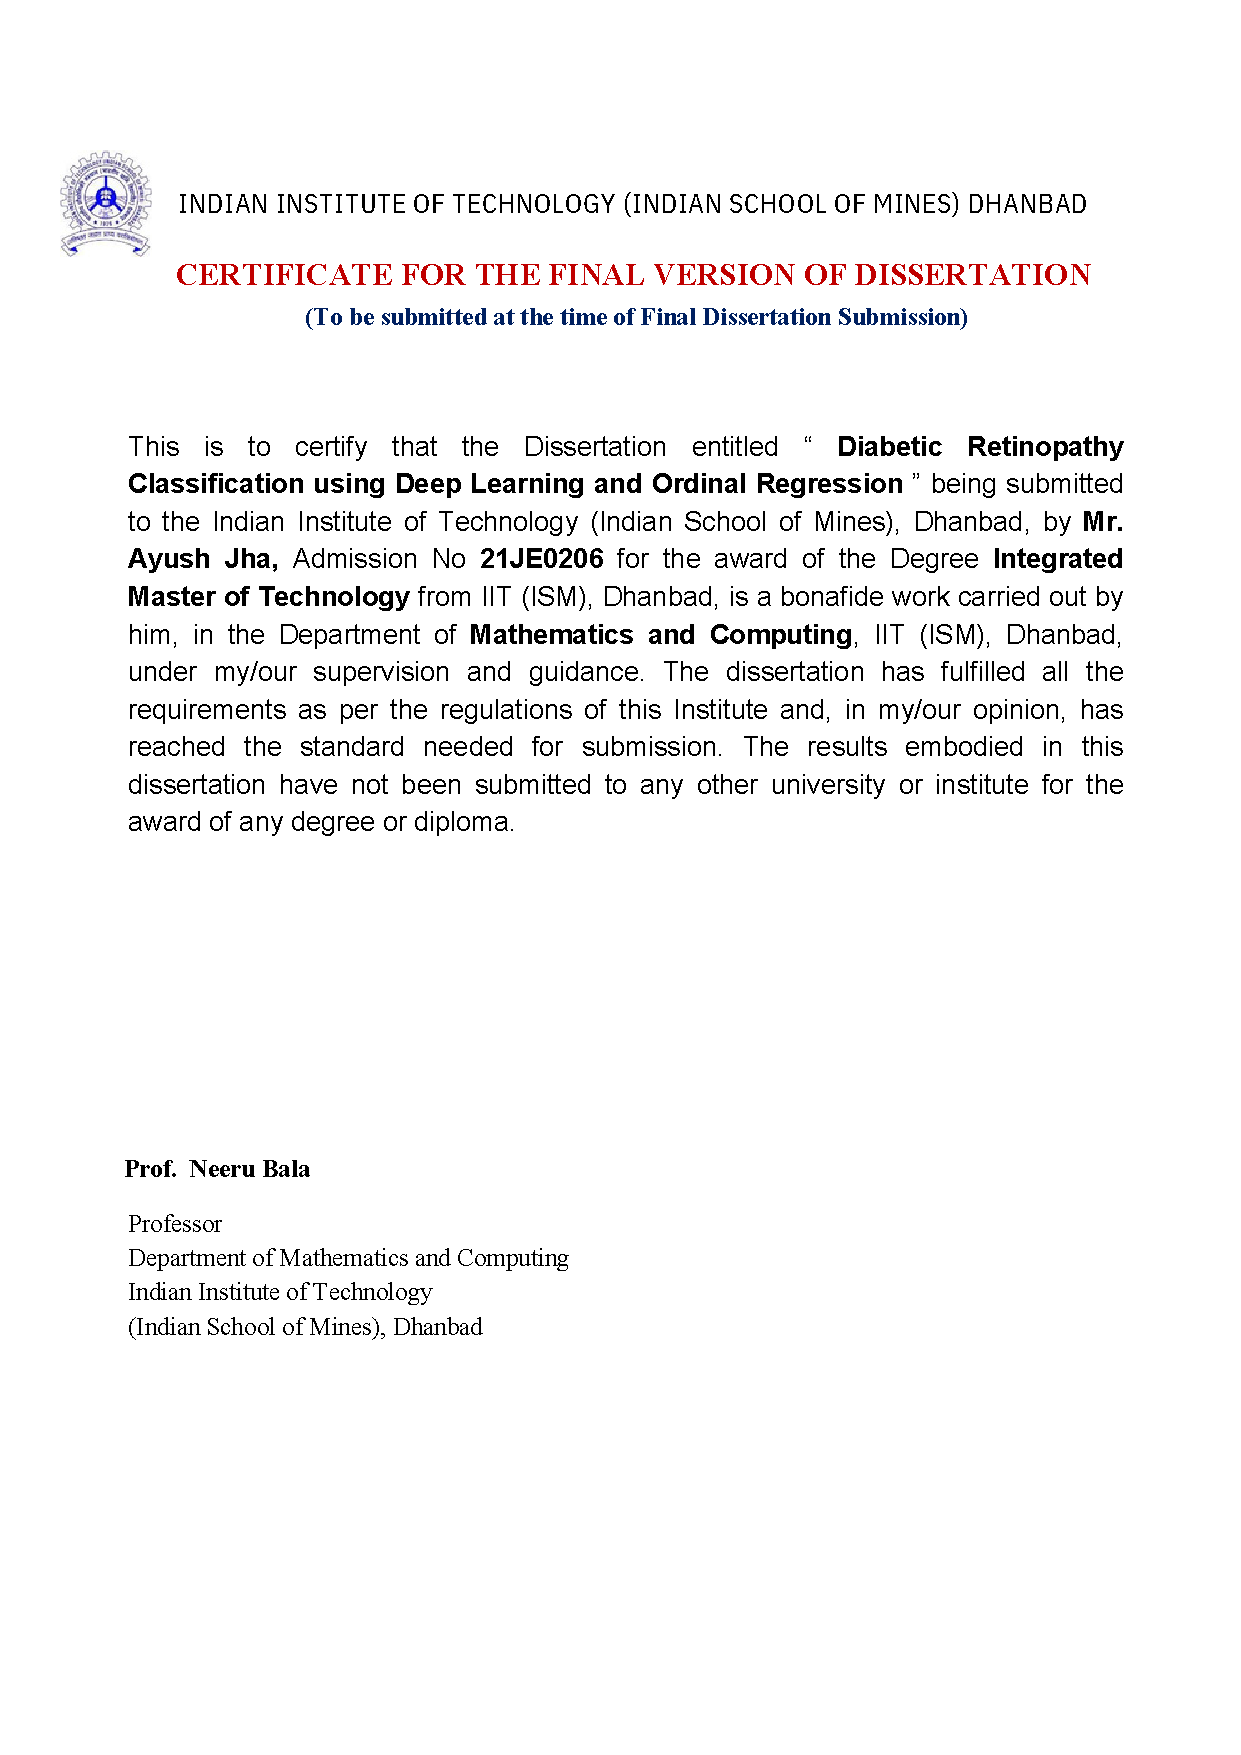
\includepdf[pages=-]{Documents.pdf}

% Acknowledgments
\chapter*{Acknowledgments}
\addcontentsline{toc}{chapter}{Acknowledgments}
I would like to express my sincere gratitude to my supervisor, \textbf{Prof.\ Neeru Bala}, for her invaluable guidance, continuous support, and encouragement throughout this research. Her expertise and constructive feedback were instrumental in shaping this work.

I am grateful to the Department of Mathematics and Computing, IIT (ISM) Dhanbad, for providing the academic environment and resources necessary for this research. I also acknowledge the Kaggle platform for providing the computational resources (GPU accelerators) that made the large-scale experiments in this thesis feasible.

Finally, I extend my heartfelt thanks to my family and friends for their unwavering support and patience during the course of this work.

\vspace{1cm}
\noindent
\textbf{Ayush Jha}\\
IIT (ISM) Dhanbad\\
May 2026

% Abstract
\clearpage
\chapter*{Abstract}
\addcontentsline{toc}{chapter}{Abstract}

Diabetic Retinopathy (DR) is a progressive microvascular complication of diabetes and a leading cause of preventable blindness worldwide. Early detection of DR severity is critical, yet manual grading is labour-intensive and subjective. This thesis investigates automated DR severity classification from fundus photographs using deep learning, focusing on ordinal regression to explicitly model the progressive nature of the disease.

We present a comparative study of three diverse architectures: (i)~EfficientNetV2-S (a CNN), (ii)~Swin Transformer V2-Tiny, and (iii)~RETFound (a foundation model adapted via LoRA). These models are evaluated within a unified framework that includes Ben Graham preprocessing, a hybrid Conditional Ordinal Regression (CORN) and Ordinal Focal Loss, and stratified five-fold cross-validation on the APTOS 2019 dataset.

By decomposing the five-class grading problem into conditional binary tasks, the ordinal framework inherently encodes clinical severity and aligns optimisation with the Quadratic Weighted Kappa (QWK) metric. All models achieve strong agreement with expert annotations: EfficientNetV2-S ($0.9116 \pm 0.0076$), Swin-V2-Tiny ($0.9074 \pm 0.0051$), and RETFound ($0.9163 \pm 0.0077$). A heterogeneous late-fusion ensemble further improves performance to a mean QWK of $\mathbf{0.9178 \pm 0.0060}$.

Our results demonstrate that domain-specific foundation models, even with minimal trainable parameters, can outperform fully fine-tuned architectures. Furthermore, the ensemble's success confirms that CNNs, transformers, and foundation models capture complementary features. This work contributes a reproducible, clinically motivated framework for ordinal DR grading and offers insights into modern medical image classification paradigms.

\vspace{0.5cm}
\noindent\textbf{Keywords:} Diabetic Retinopathy, Ordinal Regression, CORN Loss, Deep Learning, EfficientNetV2, Swin Transformer, RETFound, Foundation Models, LoRA, Ensemble Learning, Quadratic Weighted Kappa.


% Table of contents and lists
\clearpage
\begingroup
\let\clearpage\relax
\let\cleardoublepage\relax
\phantomsection
\addcontentsline{toc}{chapter}{\contentsname}
\tableofcontents

\renewcommand{\thispagestyle}[1]{} % Prevent LOF/LOT from changing the page style
\makeatletter
\renewcommand{\@mkboth}[2]{} % Prevent LOF/LOT from changing the header name
\makeatother

\setlength{\cftbeforeloftitleskip}{20pt}
\setlength{\cftafterloftitleskip}{20pt}
\setlength{\cftbeforelottitleskip}{20pt}
\setlength{\cftafterlottitleskip}{20pt}

\phantomsection
\addcontentsline{toc}{chapter}{\listfigurename}
\listoffigures

\phantomsection
\addcontentsline{toc}{chapter}{\listtablename}
\listoftables
\endgroup


\let\origcleardoublepage\cleardoublepage
\let\cleardoublepage\clearpage
\mainmatter
\let\cleardoublepage\origcleardoublepage

% Chapters
\chapter{Introduction}
\label{ch:introduction}

\section{Background and Motivation}
\label{sec:background}

Diabetes mellitus is a chronic metabolic disorder affecting an estimated 537 million adults globally as of 2021, a figure projected to rise to 783 million by 2045 \cite{teo2021global}. Among the many complications of prolonged hyperglycaemia, Diabetic Retinopathy (DR) is the most prevalent microvascular complication affecting the eyes and remains the leading cause of vision impairment and preventable blindness among the working-age population worldwide \cite{yau2012global}. DR manifests as progressive damage to the retinal vasculature, beginning with microaneurysms and intraretinal haemorrhages in its early stages and advancing to neovascularisation and tractional retinal detachment in its most severe form.

The International Clinical Diabetic Retinopathy (ICDR) severity scale, widely adopted since its standardisation by Wilkinson et al. \cite{wilkinson2003proposed}, classifies DR into five grades of increasing severity:
\begin{enumerate}[noitemsep]
    \item \textbf{Grade 0 --- No DR:} No visible retinopathy.
    \item \textbf{Grade 1 --- Mild Non-Proliferative DR (NPDR):} Presence of microaneurysms only.
    \item \textbf{Grade 2 --- Moderate NPDR:} Microaneurysms with intraretinal haemorrhages, hard exudates, or cotton-wool spots, but less severe than Grade 3.
    \item \textbf{Grade 3 --- Severe NPDR:} Extensive intraretinal haemorrhages in all four quadrants, venous beading, or prominent intraretinal microvascular abnormalities (IRMA).
    \item \textbf{Grade 4 --- Proliferative DR (PDR):} Neovascularisation of the disc or elsewhere, vitreous or preretinal haemorrhage.
\end{enumerate}

\begin{figure}[htbp]
    \centering
    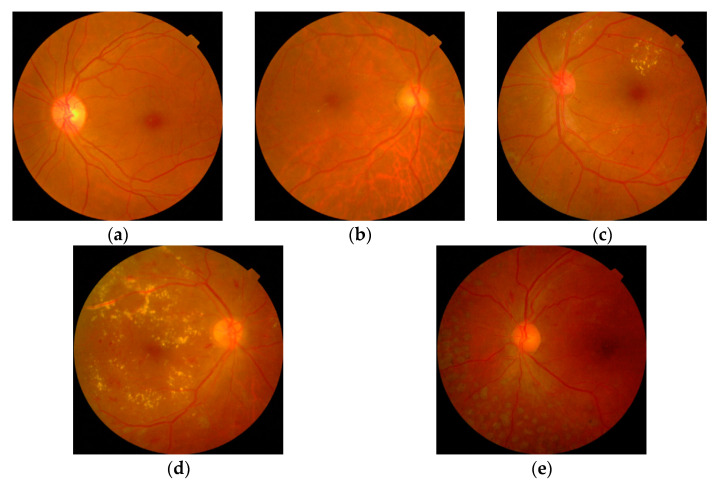
\includegraphics[width=0.8\textwidth]{diagnostics_dr_image.jpg}
    \caption{Representative fundus images illustrating the different severity grades of Diabetic Retinopathy: (a) Grade 0 (No DR), (b) Grade 1 (Mild NPDR), (c) Grade 2 (Moderate NPDR), (d) Grade 3 (Severe NPDR), and (e) Grade 4 (Proliferative DR) \cite{kassani2022diagnostics}.}
    \label{fig:diagnostics_grades}
\end{figure}

The clinical significance of this grading lies in its direct correspondence to treatment urgency. While Grades~0 and~1 generally require only routine follow-up, Grades~3 and~4 necessitate urgent referral for laser photocoagulation or intravitreal anti-VEGF therapy to prevent irreversible vision loss. Consequently, accurate and timely severity assessment is a clinical imperative.

However, the global capacity for ophthalmic screening is severely constrained. Manual grading of retinal fundus photographs by trained ophthalmologists is time-consuming, subjective (inter-grader agreement typically ranges from $\kappa = 0.65$ to $0.85$), and impractical at population scale, particularly in low- and middle-income countries where the burden of diabetes is highest yet ophthalmologist-to-patient ratios are lowest. This disparity between the scale of the screening need and the availability of expert graders provides a compelling motivation for automated, computer-aided DR classification systems.

\section{Deep Learning for Retinal Image Analysis}
\label{sec:dl_retinal}

The application of deep learning to retinal image analysis has undergone rapid evolution over the past decade. Seminal works by Gulshan et al. \cite{gulshan2016development} and Ting et al. \cite{ting2017development} demonstrated that deep convolutional neural networks (CNNs) trained on large-scale datasets of fundus photographs could achieve diagnostic accuracy comparable to, or exceeding, that of board-certified ophthalmologists for binary referable-DR detection. These studies, validated across diverse ethnic populations, established the clinical viability of AI-assisted DR screening and catalysed significant research interest.

\begin{figure}[htbp]
    \centering
    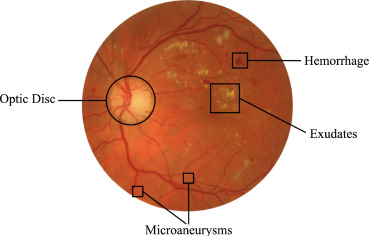
\includegraphics[width=0.8\textwidth]{bspc_dr_image.jpg}
    \caption{Illustration of deep learning methodologies and architectures applied for diabetic retinopathy detection \cite{elsevier2024bspc}.}
    \label{fig:bspc_dl_architecture}
\end{figure}

Subsequent developments in the field have been driven by three major trends. First, architectural innovation has progressed from simple transfer-learned CNNs (e.g., InceptionV3, ResNet-50) to more efficient and powerful designs such as EfficientNet \cite{tan2019efficientnet} and hierarchical vision transformers like the Swin Transformer \cite{liu2021swin}. Second, the emergence of foundation models---large-scale models pretrained on vast domain-specific corpora---has introduced a new paradigm for medical image analysis. RETFound \cite{zhou2023retfound}, pretrained on 1.6 million unlabelled retinal images via masked autoencoding, represents a notable example of this paradigm, offering strong initialisation for downstream ophthalmic tasks. Third, parameter-efficient fine-tuning methods such as Low-Rank Adaptation (LoRA) \cite{hu2022lora} have made it feasible to adapt these large foundation models to specific clinical tasks using limited labelled data and modest computational resources.

Despite these advances, a fundamental limitation persists in how the DR classification problem is typically formulated. The overwhelming majority of existing approaches treat DR grading as a nominal (unordered) multi-class classification problem, optimising standard cross-entropy loss. This formulation implicitly assumes that all misclassifications are equally costly---that confusing Grade~0 with Grade~4 is no worse than confusing Grade~1 with Grade~2. This assumption is both clinically inappropriate and mathematically incongruent with the evaluation metrics commonly used in DR grading competitions, particularly the Quadratic Weighted Kappa (QWK), which penalises misclassifications proportionally to the square of the distance between predicted and true grades.

\section{Ordinal Regression for Disease Severity Grading}
\label{sec:ordinal_motivation}

DR severity grades possess an inherent ordinal structure: Grade~0 $<$ Grade~1 $<$ Grade~2 $<$ Grade~3 $<$ Grade~4 in terms of both clinical severity and treatment urgency. Ordinal regression, unlike standard classification, explicitly models this ordering constraint. By decomposing the $K$-class ordinal problem into $K-1$ binary classification subtasks (each asking ``Is the severity greater than rank $k$?''), ordinal regression frameworks such as CORAL \cite{cao2020rank} and CORN \cite{shi2021corn} enforce rank-consistent predictions while directly aligning the training objective with distance-sensitive evaluation metrics like QWK.

This alignment is not merely a technical convenience but a clinical necessity. In a screening context, misclassifying a patient with proliferative DR (Grade~4) as having no retinopathy (Grade~0) carries far greater clinical risk than classifying them as having severe NPDR (Grade~3). Ordinal regression naturally encodes this asymmetry, making it a principled framework for disease severity grading.

\section{Research Objectives}
\label{sec:objectives}

The primary objective of this thesis is to investigate and compare deep learning architectures for DR severity classification within an ordinal regression framework. Specifically, the research contributions of this work are as follows:

\begin{enumerate}
    \item \textbf{Architectural Ablation Study:} A systematic comparison of three architecturally diverse models---a convolutional neural network (EfficientNetV2-S), a hierarchical vision transformer (Swin-V2-Tiny), and a domain-specific foundation model (RETFound with LoRA)---evaluated under identical preprocessing, training, and evaluation conditions to enable fair assessment of their relative strengths.
    
    \item \textbf{Ordinal Loss Formulation:} The design and implementation of a hybrid ordinal loss function combining Conditional Ordinal Regression (CORN) with an Ordinal Focal Loss, which simultaneously enforces rank consistency and addresses the severe class imbalance inherent in DR datasets.
    
    \item \textbf{Parameter-Efficient Foundation Model Adaptation:} A demonstration that RETFound, adapted via LoRA with only $\sim$0.4\% of its 307 million parameters trainable, can match or exceed fully fine-tuned architectures, highlighting the practical value of domain-specific pretraining.
    
    \item \textbf{Heterogeneous Ensemble Fusion:} The development of a late-fusion ensemble strategy that combines the complementary representations learned by CNN, transformer, and foundation model architectures to achieve superior and more stable performance.
    
    \item \textbf{Reproducible Experimental Framework:} A complete, open-source pipeline encompassing preprocessing, training, evaluation, and ensemble fusion, designed for reproducibility on consumer-grade GPU hardware (NVIDIA T4/P100).
\end{enumerate}


\chapter{Literature Review}
\label{ch:literature}

This chapter surveys the existing body of research relevant to the automated classification of diabetic retinopathy from retinal fundus photographs. The review is organised thematically, progressing from early handcrafted feature methods through deep convolutional approaches, modern vision transformers, and the recent emergence of foundation models for ophthalmology. Particular attention is devoted to ordinal regression techniques and ensemble strategies, as these form the methodological core of this thesis.

\section{Traditional and Early Machine Learning Approaches}
\label{sec:traditional_ml}

Prior to the deep learning era, automated DR detection relied on handcrafted feature extraction pipelines. These systems typically operated in three stages: (i)~preprocessing to enhance image quality and normalise illumination; (ii)~lesion segmentation using morphological operations, matched filters, or region growing to detect microaneurysms, haemorrhages, and exudates; and (iii)~classification using conventional machine learning algorithms such as Support Vector Machines (SVMs), Random Forests, or $k$-Nearest Neighbours.

While these approaches achieved modest accuracy on constrained datasets, they suffered from fundamental limitations. The handcrafted features were brittle to variations in imaging equipment, patient demographics, and image quality. Moreover, the multi-stage pipeline introduced cascading errors: inaccurate lesion segmentation directly degraded downstream classification performance. These limitations motivated the shift towards end-to-end deep learning approaches that learn discriminative features directly from raw pixel data.

\section{Convolutional Neural Networks for DR Classification}
\label{sec:cnn_dr}

The application of deep CNNs to DR classification was catalysed by two landmark studies. Gulshan et al. \cite{gulshan2016development} trained an Inception-V3 network on 128,175 retinal images and demonstrated performance exceeding that of ophthalmologists for binary referable-DR detection, achieving an AUC of 0.991 on the EyePACS-1 dataset. Concurrently, Ting et al. \cite{ting2017development} validated a similar approach across multiethnic populations in Singapore, achieving an AUC of 0.936 for referable DR. These studies established the clinical viability of deep learning for DR screening.

Subsequent work explored increasingly sophisticated CNN architectures. ResNet \cite{he2016deep} introduced skip connections that enabled training of very deep networks (up to 152 layers) without degradation, and became a widely adopted backbone for DR classification. The EfficientNet family \cite{tan2019efficientnet} introduced compound scaling---jointly optimising network depth, width, and input resolution---to achieve superior accuracy-efficiency trade-offs. EfficientNetV2 \cite{tan2021efficientnetv2} further improved training speed through progressive learning and the introduction of Fused-MBConv blocks, which replace the depthwise separable convolutions in early stages with conventional convolutions for improved hardware utilisation.

\subsection{Squeeze-and-Excitation and Attention Mechanisms in CNNs}

A notable development within CNN architectures has been the incorporation of channel-wise attention through Squeeze-and-Excitation (SE) blocks \cite{hu2018squeeze}. By globally pooling feature maps and learning channel-wise recalibration weights, SE blocks enable the network to emphasise informative channels and suppress less relevant ones. Both EfficientNet and EfficientNetV2 incorporate SE blocks within their MBConv building blocks, which contributes to their strong performance on fine-grained classification tasks where subtle textural differences (e.g., microaneurysms versus dot haemorrhages) are diagnostically significant.

\section{Vision Transformers for Medical Image Analysis}
\label{sec:vit_medical}

The introduction of the Vision Transformer (ViT) by Dosovitskiy et al. \cite{dosovitskiy2021image} marked a paradigm shift in computer vision. By treating an image as a sequence of non-overlapping patches and processing them with a standard Transformer encoder \cite{vaswani2017attention}, ViT demonstrated that pure self-attention architectures could achieve competitive or superior performance to CNNs on large-scale image classification benchmarks.

However, the original ViT suffered from two significant limitations for medical imaging applications. First, its quadratic computational complexity with respect to the number of patches ($\mathcal{O}(N^2)$, where $N$ is the sequence length) limited its applicability to high-resolution medical images. Second, its lack of inductive biases (e.g., translation equivariance, locality) present in CNNs made it data-hungry, requiring pretraining on hundreds of millions of images (JFT-300M) to outperform CNNs.

\subsection{Swin Transformer: Hierarchical Vision Transformers}

The Swin Transformer \cite{liu2021swin} addressed both limitations through two key innovations. First, it introduced \emph{shifted window self-attention}, which restricts the computation of self-attention to local, non-overlapping windows of fixed size, reducing the computational complexity from $\mathcal{O}(N^2)$ to $\mathcal{O}(N)$ with respect to image size. By alternating between regular and shifted window configurations across successive layers, the Swin Transformer enables cross-window information exchange while maintaining linear complexity. Second, it adopted a hierarchical architecture with progressive downsampling (patch merging), producing multi-scale feature maps analogous to those of CNNs, making it suitable for dense prediction tasks.

Swin Transformer V2 \cite{liu2022swinv2} introduced further refinements critical for scaling: (i)~\emph{post-normalisation}, which moves the LayerNorm \cite{ba2016layer} operation from before to after the attention and MLP layers to improve training stability at scale; (ii)~\emph{scaled cosine attention}, which replaces the dot-product attention with cosine similarity-based attention to prevent attention score collapse in deep networks; and (iii)~\emph{log-spaced continuous position bias (Log-CPB)}, which replaces the fixed relative position bias table with a small MLP that generates position biases from log-spaced relative coordinates, enabling smooth transfer across different window sizes and input resolutions.

\section{Foundation Models in Ophthalmology}
\label{sec:foundation_models}

The concept of foundation models---large-scale models pretrained on broad data that can be adapted to a wide range of downstream tasks---has recently been formalised by Bommasani et al. \cite{bommasani2021opportunities}. In the context of ophthalmology, RETFound \cite{zhou2023retfound}, published in \emph{Nature} in 2023, represents the first domain-specific foundation model for retinal image analysis. RETFound is a ViT-Large/16 architecture (24 Transformer blocks, 1024 embedding dimension, 16 attention heads, totalling approximately 307 million parameters) pretrained on 1.6 million unlabelled retinal images from the Moorfields Eye Hospital NHS Foundation Trust using Masked Autoencoding (MAE) \cite{he2022masked}.

The MAE pretraining strategy randomly masks a large proportion (75\%) of the input image patches and trains the model to reconstruct the missing pixels. This self-supervised objective forces the encoder to learn rich, generalisable representations of retinal morphology without requiring any labelled data. The resulting pretrained encoder serves as a powerful feature extractor that can be fine-tuned for diverse downstream tasks, including DR grading, glaucoma detection, and systemic disease prediction from retinal images.

Zhou et al. demonstrated that RETFound, when fine-tuned on relatively small labelled datasets, consistently outperformed both ImageNet-pretrained and randomly initialised models across multiple ophthalmic benchmarks. Critically, the domain-specific pretraining on retinal images provided substantial advantages over generic ImageNet pretraining, as the model had already learned to represent clinically relevant features such as vascular morphology, optic disc structure, and lesion patterns.

\subsection{Parameter-Efficient Fine-Tuning with LoRA}

Adapting foundation models with hundreds of millions of parameters to downstream tasks via full fine-tuning is computationally expensive and risks catastrophic forgetting of the pretrained representations. Low-Rank Adaptation (LoRA) \cite{hu2022lora} addresses this challenge by freezing all pretrained weights and injecting trainable rank-decomposition matrices into the attention layers. Specifically, for a pretrained weight matrix $\mathbf{W}_0 \in \mathbb{R}^{d \times k}$, LoRA constrains the weight update $\Delta\mathbf{W}$ to a low-rank decomposition:
\begin{equation}
    \mathbf{W} = \mathbf{W}_0 + \Delta\mathbf{W} = \mathbf{W}_0 + \mathbf{B}\mathbf{A}, \quad \mathbf{B} \in \mathbb{R}^{d \times r}, \quad \mathbf{A} \in \mathbb{R}^{r \times k}
\end{equation}
where $r \ll \min(d, k)$ is the adaptation rank. This reduces the number of trainable parameters from $d \times k$ to $r \times (d + k)$, typically achieving a 100--1000$\times$ reduction. For a ViT-Large with $r = 8$, injecting LoRA into the QKV projection and output projection of all 24 Transformer blocks yields approximately 1.2 million trainable parameters out of 307 million total---a reduction to roughly 0.4\% of the full parameter count.

LoRA's effectiveness in medical imaging has been extensively demonstrated. Studies have shown that LoRA-adapted foundation models can match or exceed the performance of full fine-tuning while requiring significantly less GPU memory and training time, making the foundation model paradigm accessible even on consumer-grade hardware.

\section{Ordinal Regression in Medical Image Analysis}
\label{sec:ordinal_regression_lit}

Ordinal regression---the classification of instances into ordered categories---has a long history in statistics but has only recently received sustained attention in the deep learning community. The seminal deep learning approach, CORAL (COnsistent RAnk Logits) \cite{cao2020rank}, transforms the $K$-class ordinal problem into $K-1$ binary classification tasks, each predicting $P(Y > k)$ for $k \in \{0, 1, \ldots, K-2\}$. CORAL enforces rank consistency through a \emph{weight-sharing constraint}: all $K-1$ binary classifiers share the same weight vector and differ only in their bias terms. While effective, this constraint limits model expressiveness.

CORN (Conditional Ordinal Regression for Neural Networks) \cite{shi2021corn} improved upon CORAL by achieving rank consistency without weight sharing. CORN trains each binary classifier on a \emph{conditional subset} of the data: task $k$ (predicting $P(Y > k \mid Y \geq k)$) is trained only on samples with true labels $\geq k$. By invoking the chain rule of probability, CORN guarantees monotonically non-increasing cumulative probabilities without constraining the model's representational capacity. This approach was shown to yield superior performance on ordinal classification benchmarks, particularly for tasks with many ordinal categories.

In the context of medical imaging, ordinal regression has been applied to tasks including histopathological grading, radiological severity assessment (BI-RADS), and age estimation. Recent work (2024--2025) has further validated the superiority of ordinal-aware loss functions over standard cross-entropy for medical grading tasks, with studies reporting improved quadratic weighted kappa, reduced severe misclassification rates, and better calibration of predicted severity distributions.

\section{Ensemble Methods for Classification}
\label{sec:ensemble_lit}

Ensemble methods combine the predictions of multiple models to improve accuracy and robustness beyond that achievable by any single model \cite{dietterich2000ensemble}. The theoretical basis for ensemble gains rests on the assumption that individual models make different (ideally uncorrelated) errors, allowing the ensemble to correct for individual model weaknesses through aggregation.

In the context of DR classification, heterogeneous ensembles---combining architecturally diverse models (e.g., CNNs and transformers)---are particularly promising because different architectures learn fundamentally different feature representations. CNNs excel at extracting local textural patterns (microaneurysms, dot haemorrhages) through their inherent translational equivariance and local receptive fields, while transformers capture global spatial relationships (vascular topology, optic disc-to-lesion spatial patterns) through self-attention. Foundation models, pretrained on domain-specific data, contribute representations aligned with retinal morphology that may complement both.

Late fusion, in which each model independently produces probability distributions over the severity grades and these distributions are combined through weighted averaging, is the most widely adopted ensemble strategy in medical image classification. The ensemble weights can be optimised on validation data to maximise the target metric (e.g., QWK), further amplifying the ensemble's advantage.

\section{Summary and Research Gap}
\label{sec:lit_summary}

The literature review reveals several key observations that motivate the present work:

\begin{enumerate}
    \item Most existing DR classification systems treat severity grading as nominal multi-class classification, ignoring the inherent ordinal structure of the severity scale. This leads to suboptimal alignment between the training objective and the clinical evaluation metric (QWK).
    
    \item While CNNs and vision transformers have been individually evaluated for DR classification, systematic ablation studies comparing CNN, transformer, and foundation model paradigms under identical experimental conditions remain scarce.
    
    \item The potential of parameter-efficient adaptation (LoRA) for retinal foundation models in ordinal DR grading has not been thoroughly explored.
    
    \item Heterogeneous ensembles combining these three architectural paradigms for ordinal DR classification represent an under-explored direction.
\end{enumerate}

This thesis addresses these gaps by conducting a rigorous comparative study of EfficientNetV2-S, Swin-V2-Tiny, and RETFound with LoRA, all trained within a unified ordinal regression framework, and demonstrating the benefits of their heterogeneous ensemble fusion.

\chapter{Dataset and Preprocessing}
\label{ch:dataset}

This chapter describes the dataset used for evaluation and the preprocessing pipeline applied to standardise the retinal fundus images prior to model training. Consistent preprocessing is essential for ensuring that the deep learning models focus on clinically relevant pathological features rather than artefacts of imaging variability.

\section{APTOS 2019 Blindness Detection Dataset}
\label{sec:aptos}

All experiments in this thesis are conducted on the \textbf{APTOS 2019 Blindness Detection} dataset \cite{aptos2019}, published as part of a Kaggle competition organised by the Asia Pacific Tele-Ophthalmology Society. The dataset comprises 3,662 colour fundus photographs captured across multiple clinical sites in rural India using a variety of fundus cameras. Each image is annotated by trained clinicians with a DR severity grade on the five-level ICDR scale (0--4).

\subsection{Class Distribution}

The APTOS dataset exhibits a pronounced class imbalance, as summarised in Table~\ref{tab:aptos_distribution}. The majority class (Grade~0, No DR) constitutes approximately 49.3\% of the dataset, while the minority class (Grade~4, Proliferative DR) accounts for only 5.0\%. This imbalance reflects the natural prevalence distribution of DR in screening populations and poses a significant challenge for model training, as standard loss functions tend to bias predictions towards the majority class.

\begin{table}[htbp]
\centering
\caption{Class distribution of the APTOS 2019 dataset.}
\label{tab:aptos_distribution}
\begin{tabular}{clcc}
\toprule
\textbf{Grade} & \textbf{Clinical Description} & \textbf{Count} & \textbf{Proportion (\%)} \\
\midrule
0 & No DR                    & 1,805 & 49.3 \\
1 & Mild NPDR                &   370 & 10.1 \\
2 & Moderate NPDR            &   999 & 27.3 \\
3 & Severe NPDR              &   193 &  5.3 \\
4 & Proliferative DR         &   295 &  8.1 \\
\midrule
  & \textbf{Total}           & \textbf{3,662} & \textbf{100.0} \\
\bottomrule
\end{tabular}
\end{table}

\begin{figure}[htbp]
    \centering
    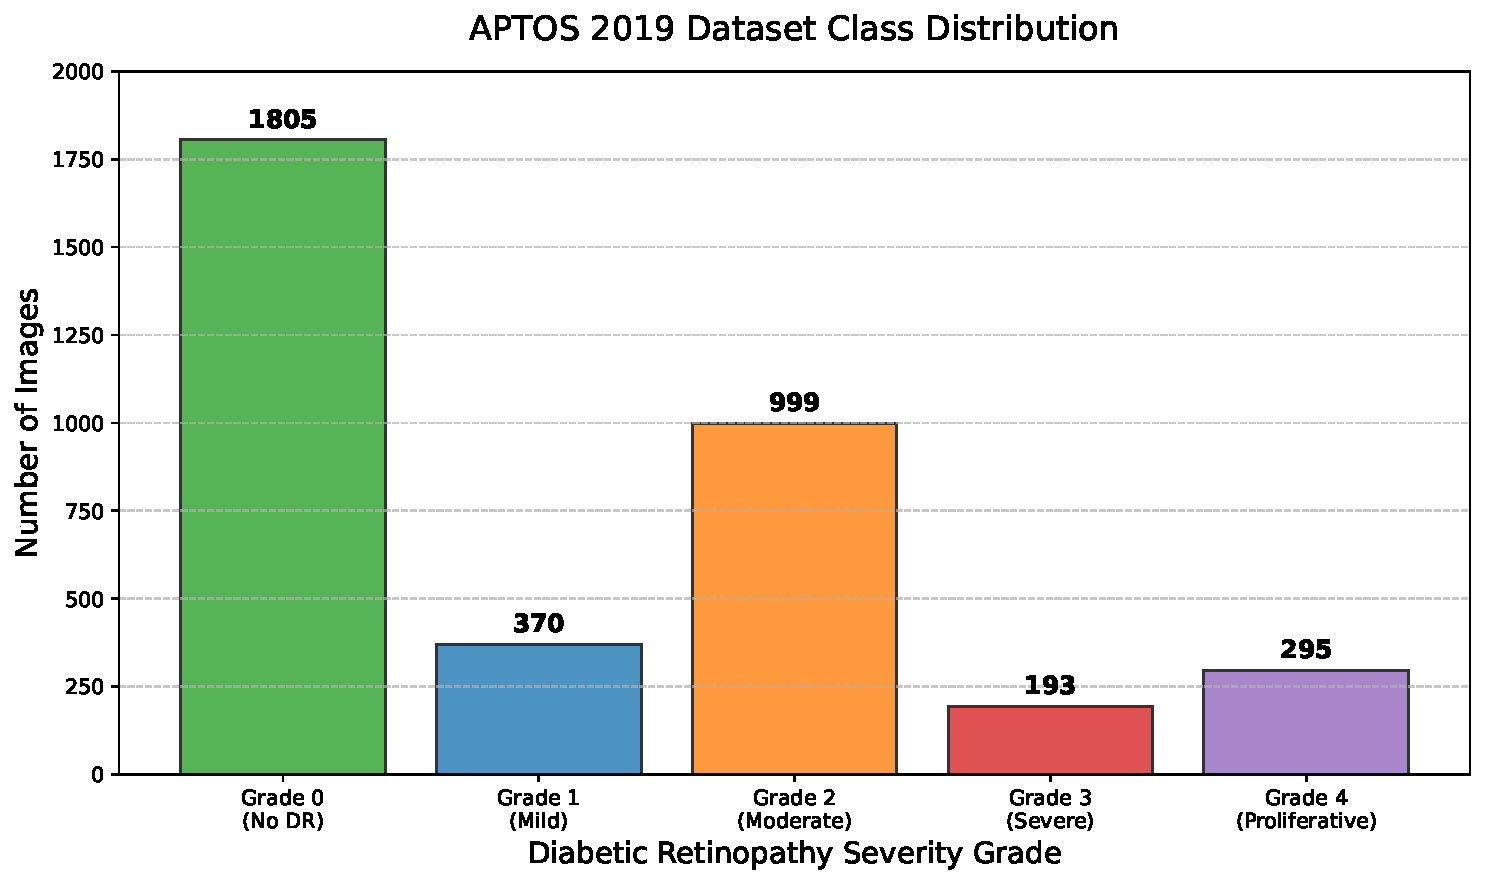
\includegraphics[width=0.7\textwidth]{eda_class_distribution}
    \caption{Exploratory Data Analysis (EDA) diagram illustrating the severe class imbalance in the APTOS 2019 dataset across the five severity grades.}
    \label{fig:eda_distribution}
\end{figure}

\subsection{Dataset Characteristics and Challenges}

The APTOS dataset presents several challenges representative of real-world clinical data:

\begin{itemize}
    \item \textbf{Imaging variability:} Images are captured with different fundus cameras, resulting in variations in resolution (ranging from $474 \times 358$ to $3,388 \times 2,588$ pixels), colour balance, contrast, and field of view.
    \item \textbf{Quality variation:} Some images exhibit poor focus, uneven illumination, dust artefacts, or significant vignetting, reflecting the challenges of tele-ophthalmology in resource-limited settings.
    \item \textbf{Annotation subjectivity:} DR grading inherently involves subjective judgement, particularly at the boundaries between adjacent grades (e.g., Grade~1 vs.~Grade~2), contributing to label noise.
    \item \textbf{Class imbalance:} The severe skew towards Grade~0 (Table~\ref{tab:aptos_distribution}) necessitates loss functions or sampling strategies that account for minority-class under-representation.
\end{itemize}

\section{Ben Graham Preprocessing Pipeline}
\label{sec:preprocessing}

To mitigate the imaging variability and enhance the discriminative quality of pathological features, we adopt a preprocessing pipeline inspired by Ben Graham's first-place solution to the 2015 Kaggle Diabetic Retinopathy Detection competition \cite{graham2015kaggle}. The pipeline comprises four sequential stages, each designed to address a specific source of variation, as illustrated in Figure~\ref{fig:preprocessing_pipeline}.

\begin{figure}[htbp]
    \centering
    \resizebox{\textwidth}{!}{%
    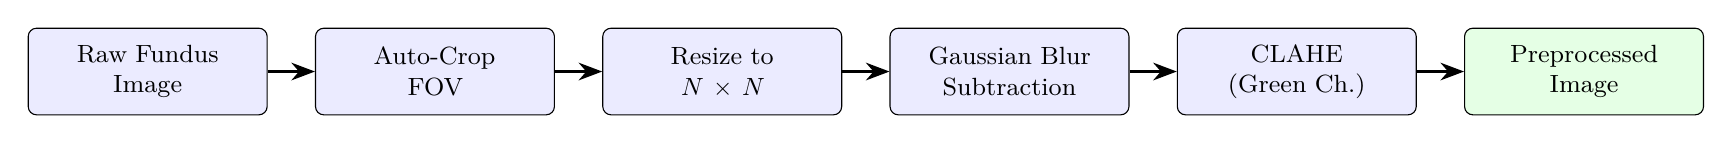
\begin{tikzpicture}[
        node distance=0.6cm,
        block/.style={rectangle, draw, fill=blue!8, text width=2.8cm, text centered, minimum height=1.1cm, rounded corners=3pt, font=\small},
        arrow/.style={-{Stealth[length=3mm]}, thick}
    ]
        \node[block] (raw) {Raw Fundus\\Image};
        \node[block, right=of raw] (crop) {Auto-Crop\\FOV};
        \node[block, right=of crop] (resize) {Resize to\\$N \times N$};
        \node[block, right=of resize] (blur) {Gaussian Blur\\Subtraction};
        \node[block, right=of blur] (clahe) {CLAHE\\(Green Ch.)};
        \node[block, right=of clahe, fill=green!10] (out) {Preprocessed\\Image};
        
        \draw[arrow] (raw) -- (crop);
        \draw[arrow] (crop) -- (resize);
        \draw[arrow] (resize) -- (blur);
        \draw[arrow] (blur) -- (clahe);
        \draw[arrow] (clahe) -- (out);
    \end{tikzpicture}%
    }
    \caption{Overview of the Ben Graham preprocessing pipeline applied to each fundus image. $N = 512$ for EfficientNetV2-S and Swin-V2-Tiny, $N = 224$ for RETFound.}
    \label{fig:preprocessing_pipeline}
\end{figure}

\subsection{Stage 1: Automated Field-of-View Cropping}
\label{sec:fov_crop}

Raw fundus images typically contain a circular field of view (FOV) surrounded by uninformative black borders. These borders vary in extent depending on the imaging equipment and contribute no diagnostic information while increasing the computational cost and potentially confusing the model. The automated cropping algorithm operates as follows:

\begin{enumerate}
    \item Convert the image to grayscale and apply a binary threshold ($\tau = 10$) to separate the bright fundus region from the dark background.
    \item Apply morphological closing with an elliptical structuring element ($15 \times 15$ pixels) to fill small gaps within the fundus region.
    \item Extract external contours and select the largest contour (corresponding to the circular FOV).
    \item Compute the bounding rectangle of this contour and crop the image with a small margin ($m = 2\%$ of the bounding box dimensions) to ensure no fundus information is lost.
\end{enumerate}

\subsection{Stage 2: Resolution Standardisation}
\label{sec:resize}

Following cropping, all images are resized to a fixed square resolution. We use $512 \times 512$ pixels for the CNN (EfficientNetV2-S) and transformer (Swin-V2-Tiny) architectures, and $224 \times 224$ pixels for the foundation model (RETFound), consistent with each model's native input resolution. Area-based interpolation is used for downsampling (to preserve anti-aliasing) and bicubic interpolation for upsampling.

\subsection{Stage 3: Gaussian Blur Subtraction}
\label{sec:gaussian_sub}

Fundus images exhibit significant low-frequency illumination variations caused by non-uniform retinal curvature, camera optics, and ambient lighting conditions. Gaussian blur subtraction removes these illumination artefacts while preserving the high-frequency pathological features (microaneurysms, haemorrhages) that are diagnostically relevant. The operation is defined as:
\begin{equation}
    I_{\text{norm}}(x, y) = I(x, y) - G_\sigma * I(x, y) + 128
    \label{eq:blur_sub}
\end{equation}
where $I(x, y)$ is the input image, $G_\sigma$ denotes a Gaussian kernel with standard deviation $\sigma = w / 30$ (where $w$ is the image width), $*$ represents convolution, and the constant 128 re-centres the pixel values to prevent negative intensities after subtraction. This operation effectively acts as a high-pass filter, normalising the local illumination while amplifying the contrast of small-scale lesions.

\subsection{Stage 4: CLAHE on the Green Channel}
\label{sec:clahe}

Contrast Limited Adaptive Histogram Equalization (CLAHE) \cite{zuiderveld1994clahe} is applied selectively to the green channel of the BGR image. The green channel is targeted because it carries the highest contrast for the haemoglobin-absorbing retinal lesions characteristic of DR (microaneurysms and haemorrhages appear as dark red structures against the orange-red fundus background, and are most visible in the green channel due to the absorption spectrum of haemoglobin).

CLAHE divides the image into a grid of non-overlapping tiles ($8 \times 8$ in our implementation) and performs histogram equalisation independently within each tile, with a clip limit ($c = 2.0$) that constrains the maximum amplification to prevent noise enhancement. The tile boundaries are interpolated bilinearly to eliminate visible seam artefacts. The enhanced green channel is then recombined with the original blue and red channels.

\subsection{Quality Filtering}
\label{sec:quality}

An optional automated quality filter is applied to identify and exclude images that are too dark (mean intensity $< 15$), too bright (mean intensity $> 245$), exhibit insufficient contrast (standard deviation $< 20$), or have an excessively small fundus region (fundus pixel ratio $< 0.15$). For the APTOS dataset, which has undergone curation, this filter rejects a negligible number of images but serves as a safeguard for more heterogeneous datasets.

\section{Data Augmentation Strategy}
\label{sec:augmentation}

To combat overfitting on the relatively small APTOS training set (approximately 2,930 images per fold after the 80/20 split), we employ a comprehensive augmentation pipeline implemented using the Albumentations library \cite{buslaev2020albumentations}. The augmentation strategy is designed to simulate the natural variability encountered in clinical fundus imaging while avoiding transformations that would alter the diagnostic content of the images.

The augmentation pipeline, applied only during training, comprises the following transformations:

\begin{itemize}
    \item \textbf{Geometric transformations:} Random resized cropping (scale: $0.8$--$1.0$, ratio: $0.9$--$1.1$), horizontal and vertical flips ($p = 0.5$ each), random 90° rotations ($p = 0.5$), and affine transformations (translation: $\pm5\%$, scaling: $0.9$--$1.1$, rotation: $\pm30°$, $p = 0.5$). These simulate variations in camera positioning and patient orientation.
    
    \item \textbf{Elastic distortions:} One of elastic transform ($\alpha = 1.0$, $\sigma = 50$), grid distortion (5 steps, limit: $0.3$), or optical distortion (limit: $0.3$) is applied with probability $p = 0.3$. These simulate the natural deformations of the curved retinal surface when projected onto a 2D image.
    
    \item \textbf{Photometric augmentations:} Random brightness and contrast adjustments ($\pm20\%$) or hue-saturation-value shifts, applied with probability $p = 0.4$. These compensate for illumination variability across imaging devices.
    
    \item \textbf{Regularisation augmentations:} Gaussian noise ($p = 0.2$), Gaussian blur ($p = 0.2$, kernel: $3$--$5$), and CoarseDropout ($p = 0.3$, 1--8 holes), which serves as a form of Cutout regularisation to improve robustness to occlusions.
\end{itemize}

During validation and evaluation, only deterministic resizing and ImageNet normalisation (mean: $[0.485, 0.456, 0.406]$, std: $[0.229, 0.224, 0.225]$) are applied to ensure reproducibility.

\section{Cross-Validation Protocol}
\label{sec:cv}

To obtain robust performance estimates, we employ \textbf{stratified 5-fold cross-validation} \cite{refaeilzadeh2009cross} with a fixed random seed ($s = 42$). Stratification ensures that the class distribution in each fold mirrors the overall dataset distribution, which is particularly important given the severe class imbalance (Table~\ref{tab:aptos_distribution}). Each fold uses approximately 80\% of the data (2,930 images) for training and 20\% (732 images) for validation. All three models and the ensemble are evaluated on identical fold splits to enable fair comparison.

\chapter{Methodology}
\label{ch:methodology}

This chapter presents the technical methodology underlying the three deep learning architectures, the ordinal regression loss formulation, and the ensemble fusion strategy. Each model shares a common CORN ordinal classification head and hybrid loss function but differs fundamentally in its feature extraction backbone, representing the CNN, transformer, and foundation model paradigms respectively.


\section{CORN Ordinal Label Encoding and Decoding}
\label{sec:corn_encoding}

Central to the ordinal regression framework employed in this thesis is the encoding of the five-level DR severity grade into a binary ordinal representation compatible with the Conditional Ordinal Regression (CORN) framework \cite{shi2021corn}.

\subsection{Label Encoding}

For $K = 5$ ordinal classes, CORN defines $K - 1 = 4$ binary classification tasks. Each task $k \in \{0, 1, 2, 3\}$ answers the question: \emph{``Is the DR severity strictly greater than rank $k$?''} Given a true grade $y \in \{0, 1, 2, 3, 4\}$, the binary ordinal target vector $\mathbf{c} \in \{0, 1\}^{4}$ is constructed as:
\begin{equation}
    c_k = \mathbb{1}[y > k], \quad k \in \{0, 1, 2, 3\}
    \label{eq:corn_encode}
\end{equation}

This encoding produces monotonically non-increasing binary vectors. For example:
\begin{align*}
    \text{Grade } 0 &\rightarrow [0, 0, 0, 0] \\
    \text{Grade } 1 &\rightarrow [1, 0, 0, 0] \\
    \text{Grade } 2 &\rightarrow [1, 1, 0, 0] \\
    \text{Grade } 3 &\rightarrow [1, 1, 1, 0] \\
    \text{Grade } 4 &\rightarrow [1, 1, 1, 1]
\end{align*}

\subsection{Prediction Decoding}

At inference time, the model outputs $K - 1 = 4$ logits. The predicted grade is obtained by applying the sigmoid function to each logit, thresholding at 0.5, and counting the number of consecutive positive predictions:
\begin{equation}
    \hat{y} = \sum_{k=0}^{K-2} \mathbb{1}\left[\sigma(z_k) > 0.5\right]
    \label{eq:corn_decode}
\end{equation}
where $z_k$ is the $k$-th logit and $\sigma(\cdot)$ is the sigmoid function. This decoding naturally produces integer predictions in $\{0, 1, \ldots, K-1\}$.

\subsection{Probability Conversion}

For ensemble fusion (Section~\ref{sec:ensemble_method}), the ordinal logits must be converted to $K$-class probability distributions. Defining $\hat{p}_k = \sigma(z_k)$ as the estimated cumulative exceedance probability for rank $k$, the class probabilities are computed as:
\begin{equation}
    P(Y = j) = \begin{cases}
        1 - \hat{p}_0 & \text{if } j = 0 \\
        \hat{p}_{j-1} - \hat{p}_j & \text{if } 1 \leq j \leq K-2 \\
        \hat{p}_{K-2} & \text{if } j = K-1
    \end{cases}
    \label{eq:corn_probs}
\end{equation}
These probabilities are clipped to $[0, 1]$ and renormalised to ensure a valid probability distribution.

\section{Model A: EfficientNetV2-S}
\label{sec:model_a}

\subsection{Architecture Overview}

EfficientNetV2-S \cite{tan2021efficientnetv2} serves as the CNN baseline in our ablation study, representing the state of the art in efficient convolutional architecture design. It belongs to the EfficientNetV2 family, which improves upon the original EfficientNet \cite{tan2019efficientnet} through three key innovations: (i)~the introduction of Fused-MBConv blocks in early stages, (ii)~progressive learning during training, and (iii)~a refined Neural Architecture Search (NAS) procedure that jointly optimises accuracy and training speed.

\begin{figure}[htbp]
    \centering
    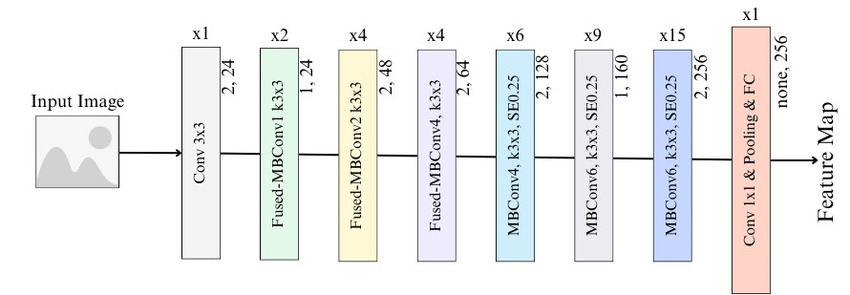
\includegraphics[width=0.8\textwidth]{arch_efficientnetv2.jpeg}
    \caption{Architecture of EfficientNetV2-S. The network consists of a sequence of MBConv and Fused-MBConv stages with progressive channel expansion, followed by global average pooling.}
    \label{fig:efficientnetv2_arch}
\end{figure}

\subsection{Building Blocks}

The EfficientNetV2-S architecture employs two types of inverted residual blocks:

\textbf{Fused-MBConv} blocks, used in the early stages (Stages 1--3), replace the depthwise separable convolution with a single fused $3 \times 3$ convolution for both spatial and channel mixing. This design improves hardware utilisation on modern accelerators (GPUs/TPUs) where memory access costs dominate over computation for depthwise convolutions. The Fused-MBConv operation for input $\mathbf{X}$ can be expressed as:
\begin{equation}
    \mathbf{Y} = \text{SE}\left(\text{BN}\left(\text{GELU}\left(\text{Conv}_{3\times3}^{e \cdot c}(\mathbf{X})\right)\right)\right) + \mathbf{X}
\end{equation}
where $c$ is the input channel count, $e$ is the expansion ratio, $\text{BN}$ denotes batch normalisation, and $\text{SE}$ denotes the squeeze-and-excitation block \cite{hu2018squeeze}.

\textbf{MBConv} blocks \cite{sandler2018mobilenetv2}, used in the later stages (Stages 4--7), employ the standard depthwise separable convolution:
\begin{equation}
    \mathbf{Y} = \text{SE}\left(\text{BN}\left(\text{DWConv}_{3\times3}\left(\text{BN}\left(\text{GELU}\left(\text{Conv}_{1\times1}^{e \cdot c}(\mathbf{X})\right)\right)\right)\right)\right) + \mathbf{X}
\end{equation}
where $\text{DWConv}$ is a depthwise convolution that applies a single filter per input channel, reducing computation by a factor of $c$ compared to standard convolutions.

\subsection{Classification Head}

The convolutional feature maps from the final stage are reduced to a 1280-dimensional feature vector via global average pooling. This vector is passed through a CORN ordinal head consisting of:
\begin{equation}
    \hat{\mathbf{z}} = \mathbf{W}_{\text{corn}} \cdot \text{Dropout}\left(\text{LayerNorm}(\mathbf{f})\right) + \mathbf{b}_{\text{corn}}
\end{equation}
where $\mathbf{f} \in \mathbb{R}^{1280}$ is the pooled feature vector, $\mathbf{W}_{\text{corn}} \in \mathbb{R}^{4 \times 1280}$, and the output $\hat{\mathbf{z}} \in \mathbb{R}^{4}$ represents the four ordinal logits. LayerNorm is applied before the linear projection to stabilise the feature magnitudes, and dropout ($p = 0.15$) provides regularisation.

\section{Model B: Swin Transformer V2-Tiny}
\label{sec:model_b}

\subsection{Architecture Overview}

The Swin Transformer V2-Tiny \cite{liu2022swinv2} represents the hierarchical vision transformer paradigm in our study. Unlike the CNN baseline that builds representations through local convolutions, the Swin Transformer captures global spatial dependencies through self-attention while maintaining computational efficiency via the shifted window mechanism.

\begin{figure}[htbp]
    \centering
    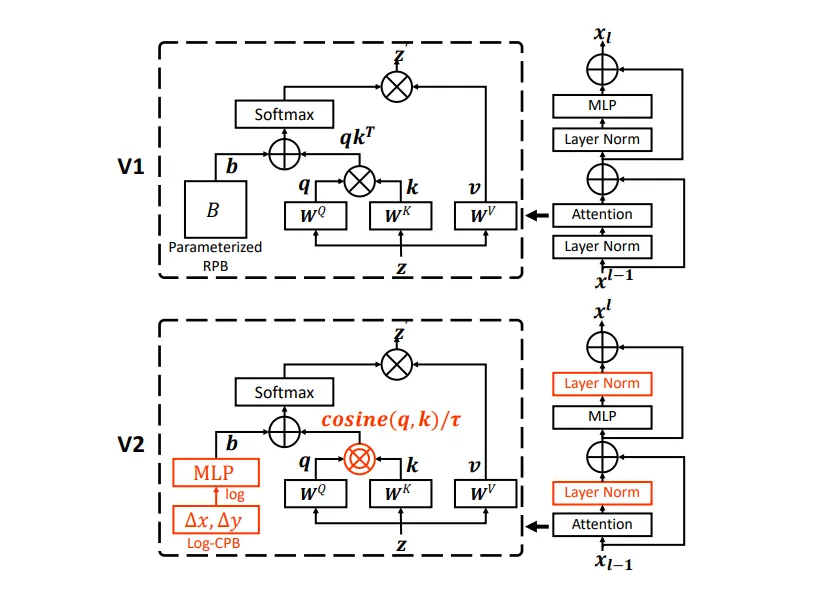
\includegraphics[width=0.8\textwidth]{arch_swinv2.jpg}
    \caption{Architecture of Swin Transformer V2. The model processes images through four hierarchical stages with progressive spatial downsampling and channel expansion. Within each stage, attention is computed within local windows that alternate between regular and shifted configurations \cite{chuah2024swinarch}.}
    \label{fig:swinv2_arch}
\end{figure}

\subsection{Shifted Window Self-Attention}

The core innovation of the Swin Transformer is the restriction of self-attention computation to non-overlapping local windows of size $M \times M$ (with $M = 8$ in our configuration). For an input feature map of spatial resolution $H \times W$, standard global self-attention has complexity $\mathcal{O}(H^2W^2)$, while window-based attention reduces this to $\mathcal{O}(HWM^2)$---linear in image size.

To enable cross-window information exchange, successive Transformer layers alternate between two windowing configurations. In odd-numbered layers, the windows are regularly partitioned; in even-numbered layers, the window grid is shifted by $(\lfloor M/2 \rfloor, \lfloor M/2 \rfloor)$ pixels, causing each shifted window to overlap with four regular windows from the previous layer. This shifted configuration is implemented efficiently using cyclic shifting and attention masking, avoiding any actual data movement.

The attention computation within each window follows the scaled dot-product formulation. In Swin-V2, the standard dot-product attention is replaced with \emph{scaled cosine attention}:
\begin{equation}
    \text{Attention}(\mathbf{Q}, \mathbf{K}, \mathbf{V}) = \text{softmax}\left(\frac{\cos(\mathbf{Q}, \mathbf{K})}{\tau} + \mathbf{B}\right)\mathbf{V}
    \label{eq:cosine_attention}
\end{equation}
where $\tau$ is a learnable temperature parameter and $\mathbf{B}$ is a relative position bias generated by a log-spaced continuous position bias (Log-CPB) MLP.

\subsection{Hierarchical Feature Maps}

The Swin-V2-Tiny architecture comprises four stages, with patch merging layers between them that halve the spatial resolution while doubling the channel dimension:

\begin{itemize}
    \item \textbf{Stage 1:} Patch embedding ($4 \times 4$ patches, $C = 96$) followed by 2 Transformer blocks.
    \item \textbf{Stage 2:} Patch merging ($2\times$ downsample, $2C = 192$) followed by 2 Transformer blocks.
    \item \textbf{Stage 3:} Patch merging ($2\times$ downsample, $4C = 384$) followed by 6 Transformer blocks.
    \item \textbf{Stage 4:} Patch merging ($2\times$ downsample, $8C = 768$) followed by 2 Transformer blocks.
\end{itemize}

The output of Stage~4 is a $768$-dimensional feature vector obtained via LayerNorm followed by adaptive average pooling. This feature vector is passed through the same CORN ordinal head architecture described in Section~\ref{sec:model_a}, with dropout $p = 0.20$ (increased for the transformer due to its higher overfitting tendency on small datasets).

\section{Model D: RETFound with LoRA}
\label{sec:model_d}

\subsection{Architecture Overview}

RETFound \cite{zhou2023retfound} is a Vision Transformer Large (ViT-L/16) pretrained on 1.6 million colour fundus photographs from the Moorfields Eye Hospital via Masked Autoencoding (MAE) \cite{he2022masked}. It operates on $224 \times 224$ images, dividing each image into a grid of $14 \times 14 = 196$ non-overlapping patches of size $16 \times 16$ pixels. Each patch is linearly projected to a 1024-dimensional embedding, and a learnable \texttt{[CLS]} token is prepended, yielding a sequence of 197 tokens.

The encoder consists of 24 Transformer blocks, each containing multi-head self-attention (16 heads, head dimension 64) and an MLP with GELU activation and expansion ratio 4. Learnable absolute position embeddings are added to the patch sequence. The \texttt{[CLS]} token output from the final block serves as the global image representation.

\begin{figure}[htbp]
    \centering
    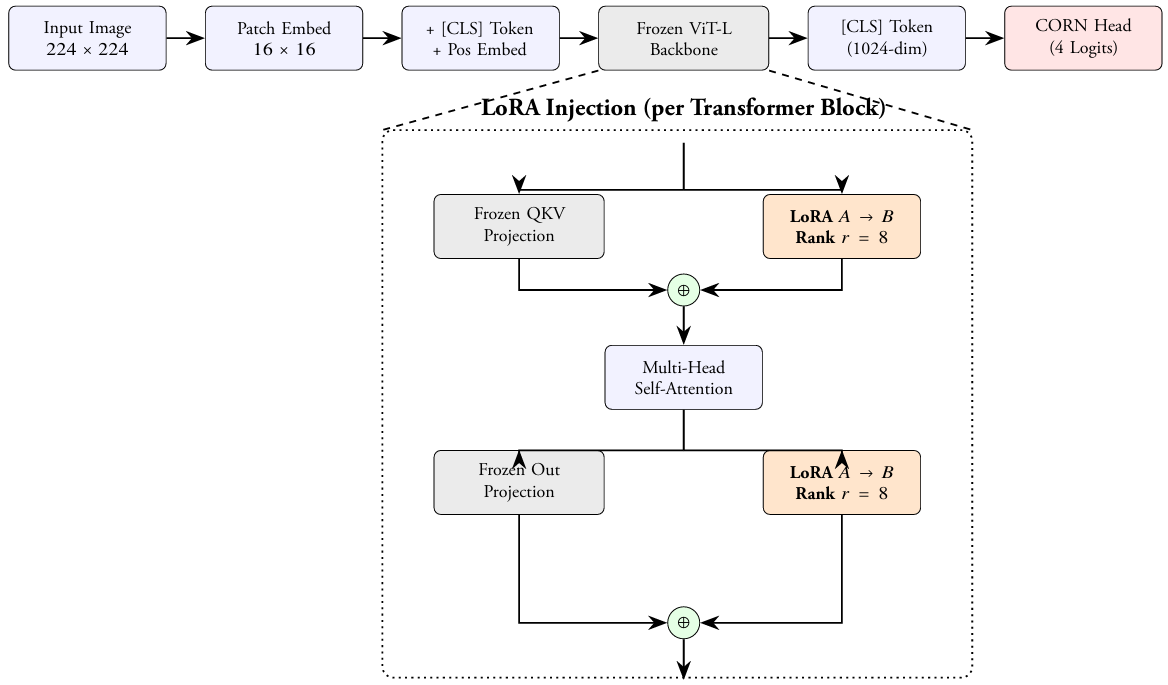
\includegraphics[width=0.8\textwidth]{arch_Retfound.png}
    \caption{Architecture overview of RETFound, a Vision Transformer (ViT-Large) foundation model pretrained via Masked Autoencoding on 1.6 million retinal images.}
    \label{fig:retfound_arch}
\end{figure}

\subsection{LoRA Injection Strategy}

Rather than fine-tuning the full 307 million parameters of RETFound (which risks catastrophic forgetting and exceeds the VRAM capacity of consumer GPUs), we freeze all pretrained backbone weights and inject LoRA adapters \cite{hu2022lora} into the self-attention layers of every Transformer block.

For each target linear layer $\mathbf{W}_0 \in \mathbb{R}^{d_{\text{out}} \times d_{\text{in}}}$, the LoRA modification is:
\begin{equation}
    \mathbf{h} = \mathbf{W}_0 \mathbf{x} + \frac{\alpha}{r} \cdot \mathbf{B}\mathbf{A}\mathbf{x}
    \label{eq:lora_forward}
\end{equation}
where $\mathbf{A} \in \mathbb{R}^{r \times d_{\text{in}}}$ and $\mathbf{B} \in \mathbb{R}^{d_{\text{out}} \times r}$ are the low-rank trainable matrices, $r = 8$ is the adaptation rank, and $\alpha = 16$ is the scaling factor. The matrix $\mathbf{A}$ is initialised with Kaiming uniform initialisation and $\mathbf{B}$ is initialised to zero, ensuring that the LoRA contribution is zero at the start of training and the model begins from the pretrained state.

LoRA is injected into two target modules per Transformer block:
\begin{enumerate}
    \item The \textbf{QKV projection} ($\mathbf{W}_{\text{qkv}} \in \mathbb{R}^{3072 \times 1024}$): a fused linear layer that jointly computes the query, key, and value projections for all attention heads.
    \item The \textbf{output projection} ($\mathbf{W}_{\text{proj}} \in \mathbb{R}^{1024 \times 1024}$): the linear layer that projects the concatenated multi-head attention output back to the embedding dimension.
\end{enumerate}

With 24 Transformer blocks $\times$ 2 LoRA modules per block $= 48$ LoRA layers, and each LoRA layer introducing $r \times (d_{\text{in}} + d_{\text{out}})$ parameters, the total trainable parameter count is approximately 1.2 million out of 307 million ($\sim$0.4\%). The CORN classification head adds an additional $\sim$4,100 trainable parameters.

A LoRA dropout of $p = 0.05$ is applied to the input $\mathbf{x}$ before the low-rank projection to regularise the adaptation and reduce overfitting on the small APTOS dataset.

\subsection{Gradient Checkpointing}

To accommodate the ViT-Large backbone within the 16~GB VRAM constraint of NVIDIA T4 GPUs, we employ gradient checkpointing \cite{chen2016training} during training. Rather than storing the activations of all 24 Transformer blocks for the backward pass, gradient checkpointing stores activations only at designated checkpoints and recomputes intermediate activations during backpropagation. This trades a moderate increase in computation time ($\sim$30\%) for a substantial reduction in peak memory usage, enabling training with batch size 4 on a single T4 GPU.

\section{Hybrid Ordinal Loss Function}
\label{sec:loss_function}

A key contribution of this thesis is the design of a hybrid loss function that combines the ordinal consistency of CORN with the class-imbalance handling of Focal Loss. The total loss is defined as:
\begin{equation}
    \mathcal{L}_{\text{total}} = \alpha \cdot \mathcal{L}_{\text{CORN}} + (1 - \alpha) \cdot \mathcal{L}_{\text{Focal}}
    \label{eq:hybrid_loss}
\end{equation}
where $\alpha = 0.7$ balances the two components, placing primary emphasis on ordinal consistency while retaining the benefits of focal down-weighting.

\subsection{CORN Loss}
\label{sec:corn_loss}

The CORN loss \cite{shi2021corn} achieves rank consistency through conditional training. For each rank $k \in \{0, 1, \ldots, K-2\}$, a binary cross-entropy loss is computed \emph{only on the conditional subset of samples where the true grade $y \geq k$}:
\begin{equation}
    \mathcal{L}_{\text{CORN}} = \frac{1}{|\mathcal{K}|} \sum_{k \in \mathcal{K}} \frac{1}{|\mathcal{S}_k|} \sum_{i \in \mathcal{S}_k} \text{BCE}\left(z_k^{(i)}, \, \mathbb{1}[y^{(i)} > k]\right)
    \label{eq:corn_loss}
\end{equation}
where $\mathcal{S}_k = \{i : y^{(i)} \geq k\}$ is the conditional training set for task $k$, $\mathcal{K}$ is the set of ranks with non-empty conditional sets, $z_k^{(i)}$ is the $k$-th logit for sample $i$, and $\text{BCE}$ is the binary cross-entropy:
\begin{equation}
    \text{BCE}(z, t) = -\left[t \log \sigma(z) + (1-t) \log(1 - \sigma(z))\right]
\end{equation}

The conditioning ensures that task $k$ learns the probability $P(Y > k \mid Y \geq k)$ rather than $P(Y > k)$. By the chain rule of probability, the cumulative probabilities $P(Y > k) = \prod_{j=0}^{k} P(Y > j \mid Y \geq j)$ are guaranteed to be monotonically non-increasing, ensuring rank-consistent predictions without requiring the weight-sharing constraint of CORAL.

\subsection{Ordinal Focal Loss}
\label{sec:focal_loss}

The Ordinal Focal Loss extends the standard Focal Loss \cite{lin2017focal} to the ordinal binary structure of CORN. Applied across all $K-1$ binary tasks simultaneously, it down-weights well-classified ordinal transitions and focuses learning on the difficult boundary grades:
\begin{equation}
    \mathcal{L}_{\text{Focal}} = \frac{1}{B \cdot (K-1)} \sum_{i=1}^{B} \sum_{k=0}^{K-2} -\alpha_t^{(i,k)} \left(1 - p_t^{(i,k)}\right)^\gamma \log\left(p_t^{(i,k)}\right)
    \label{eq:focal_loss}
\end{equation}
where $B$ is the batch size, $p_t^{(i,k)}$ is the predicted probability for the correct binary outcome at rank $k$:
\begin{equation}
    p_t^{(i,k)} = c_k^{(i)} \cdot \sigma(z_k^{(i)}) + (1 - c_k^{(i)}) \cdot (1 - \sigma(z_k^{(i)}))
\end{equation}
$\gamma = 2.0$ is the focusing parameter that controls the rate of down-weighting for easy examples, and $\alpha_t^{(i,k)}$ is a class-balancing factor ($\alpha = 0.25$ for positive, $1 - \alpha = 0.75$ for negative outcomes).

\subsection{Rationale for the Hybrid Formulation}

The two loss components serve complementary purposes. CORN loss ensures that the model's ordinal predictions are rank-consistent and that the training objective is aligned with the QWK evaluation metric, which penalises misclassifications proportionally to the squared distance between predicted and true grades. The Ordinal Focal Loss addresses the class imbalance by reducing the contribution of well-classified (easy) ordinal transitions, directing the model's capacity towards the challenging boundary cases (e.g., distinguishing Grade~1 from Grade~2). The weight $\alpha = 0.7$ reflects the higher priority placed on ordinal consistency.

\section{Quadratic Weighted Kappa}
\label{sec:qwk}

The Quadratic Weighted Kappa (QWK) \cite{cohen1968weighted} is adopted as the primary evaluation metric, consistent with the APTOS 2019 competition and clinical DR grading practice. QWK measures the agreement between the predicted grades $\hat{y}$ and the true grades $y$, adjusted for agreement expected by chance, with a quadratic weighting scheme that penalises large disagreements more heavily.

Given the confusion matrix $\mathbf{O}$ (observed) and the expected matrix $\mathbf{E}$ (under random agreement), the QWK is defined as:
\begin{equation}
    \kappa_w = 1 - \frac{\sum_{i,j} w_{ij} \cdot O_{ij}}{\sum_{i,j} w_{ij} \cdot E_{ij}}
    \label{eq:qwk}
\end{equation}
where the quadratic weight matrix is:
\begin{equation}
    w_{ij} = \frac{(i - j)^2}{(K - 1)^2}
    \label{eq:qwk_weights}
\end{equation}

QWK ranges from $-1$ (complete disagreement) through $0$ (chance agreement) to $+1$ (perfect agreement). Values above 0.80 are generally considered ``almost perfect agreement'' in clinical contexts. The quadratic weighting makes QWK particularly appropriate for ordinal classification because it imposes zero penalty for correct predictions, mild penalty for off-by-one errors, and severe penalty for distant misclassifications---directly mirroring the clinical severity of grading errors.

\section{Heterogeneous Late-Fusion Ensemble}
\label{sec:ensemble_method}

The three trained models produce different feature representations that capture complementary aspects of retinal pathology. To exploit this complementarity, we employ a heterogeneous late-fusion ensemble that combines the class probability distributions from all three models through optimised weighted averaging.

\begin{figure}[htbp]
    \centering
    \resizebox{\textwidth}{!}{%
    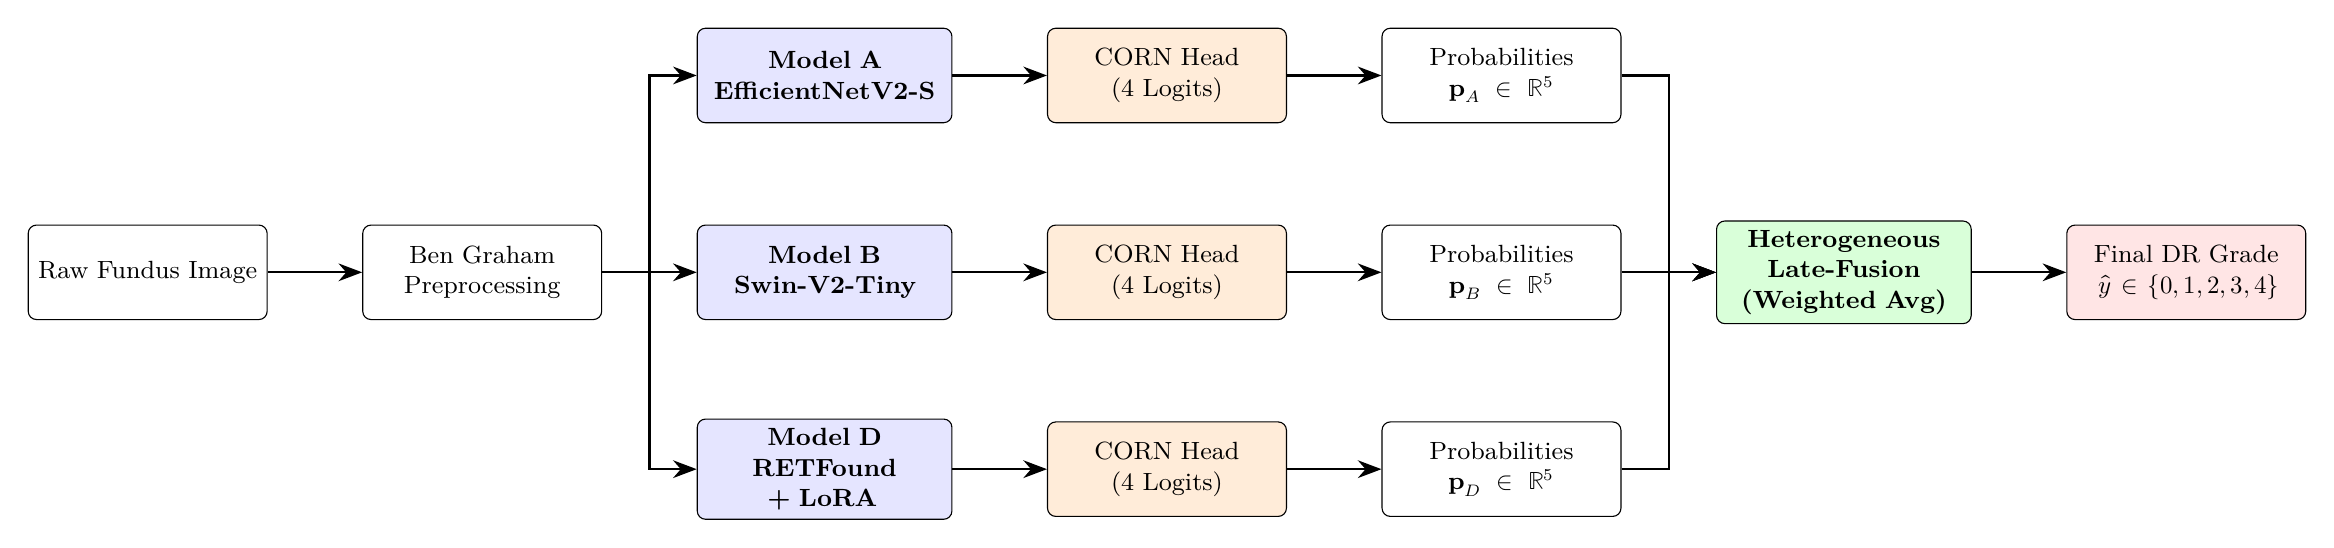
\begin{tikzpicture}[
        node distance=0.8cm and 1.2cm,
        auto,
        box/.style={rectangle, draw, fill=white, text width=2.8cm, text centered, minimum height=1.2cm, rounded corners=3pt, font=\small},
        modelbox/.style={rectangle, draw, fill=blue!10, text width=3cm, text centered, minimum height=1.2cm, rounded corners=3pt, font=\small\bfseries},
        cornbox/.style={rectangle, draw, fill=orange!15, text width=2.8cm, text centered, minimum height=1.2cm, rounded corners=3pt, font=\small},
        fusionbox/.style={rectangle, draw, fill=green!15, text width=3cm, text centered, minimum height=1.2cm, rounded corners=3pt, font=\small\bfseries},
        arrow/.style={-{Stealth[length=3mm]}, thick}
    ]
        % Nodes
        \node[box] (input) {Raw Fundus Image};
        \node[box, right=of input] (preprocess) {Ben Graham Preprocessing};
        
        \node[modelbox, right=of preprocess, yshift=2.5cm] (modelA) {Model A\\EfficientNetV2-S};
        \node[modelbox, right=of preprocess] (modelB) {Model B\\Swin-V2-Tiny};
        \node[modelbox, right=of preprocess, yshift=-2.5cm] (modelD) {Model D\\RETFound + LoRA};
        
        \node[cornbox, right=of modelA] (cornA) {CORN Head\\(4 Logits)};
        \node[cornbox, right=of modelB] (cornB) {CORN Head\\(4 Logits)};
        \node[cornbox, right=of modelD] (cornD) {CORN Head\\(4 Logits)};
        
        \node[box, right=of cornA] (probA) {Probabilities\\$\mathbf{p}_A \in \mathbb{R}^5$};
        \node[box, right=of cornB] (probB) {Probabilities\\$\mathbf{p}_B \in \mathbb{R}^5$};
        \node[box, right=of cornD] (probD) {Probabilities\\$\mathbf{p}_D \in \mathbb{R}^5$};
        
        \node[fusionbox, right=of probB] (fusion) {Heterogeneous Late-Fusion\\(Weighted Avg)};
        
        \node[box, fill=red!10, right=of fusion] (output) {Final DR Grade\\$\hat{y} \in \{0,1,2,3,4\}$};
        
        % Arrows
        \draw[arrow] (input) -- (preprocess);
        \draw[arrow] (preprocess.east) -- ++(0.6,0) |- (modelA.west);
        \draw[arrow] (preprocess.east) -- (modelB.west);
        \draw[arrow] (preprocess.east) -- ++(0.6,0) |- (modelD.west);
        
        \draw[arrow] (modelA) -- (cornA);
        \draw[arrow] (modelB) -- (cornB);
        \draw[arrow] (modelD) -- (cornD);
        
        \draw[arrow] (cornA) -- (probA);
        \draw[arrow] (cornB) -- (probB);
        \draw[arrow] (cornD) -- (probD);
        
        \draw[arrow] (probA.east) -- ++(0.6,0) |- (fusion.west);
        \draw[arrow] (probB.east) -- (fusion.west);
        \draw[arrow] (probD.east) -- ++(0.6,0) |- (fusion.west);
        
        \draw[arrow] (fusion) -- (output);
        
    \end{tikzpicture}%
    }
    \caption{End-to-end methodology pipeline. Raw fundus images undergo Ben Graham preprocessing before being passed to three distinct architectures (CNN, Transformer, Foundation Model). Each model features a Conditional Ordinal Regression (CORN) head. The resulting logits are converted to class probabilities and fused via a weighted average to produce the final DR severity grade.}
    \label{fig:overall_pipeline}
\end{figure}
\subsection{Fusion Strategy}

For each validation fold, the CORN logits from each model are first converted to $K$-class probability distributions using Equation~\ref{eq:corn_probs}. The fused probability distribution is then computed as:
\begin{equation}
    \mathbf{p}_{\text{ens}} = \sum_{m=1}^{M} w_m \cdot \mathbf{p}_m, \quad \text{subject to} \quad \sum_{m=1}^{M} w_m = 1, \quad w_m \geq 0
    \label{eq:ensemble_fusion}
\end{equation}
where $M = 3$ is the number of models, $\mathbf{p}_m \in \mathbb{R}^K$ is the probability vector from model $m$, and $w_m$ is the fusion weight for model $m$.

\subsection{Weight Optimisation}

The fusion weights are optimised per fold via grid search to maximise the QWK on the validation set. For three models, we use a pair-wise iterative optimisation strategy with 21 grid steps per dimension, evaluating all feasible weight combinations that satisfy the simplex constraint. This procedure independently selects the optimal weight configuration for each fold, allowing the ensemble to adapt to fold-specific model strengths.

\chapter{Experimental Setup}
\label{ch:experimental}

This chapter specifies the hardware, software, hyperparameters, and training procedures used to conduct the experiments reported in this thesis.

\section{Hardware and Software Environment}
\label{sec:hardware}

All model training and evaluation were conducted on the Kaggle platform using NVIDIA GPU accelerators. Depending on session allocation, either an NVIDIA Tesla T4 (16~GB VRAM, Turing architecture) or an NVIDIA Tesla P100 (16~GB VRAM, Pascal architecture) was used. The training pipeline was implemented in Python 3.10 using PyTorch 2.x as the deep learning framework, with torchvision for pretrained model weights, Albumentations \cite{buslaev2020albumentations} for data augmentation, and scikit-learn for metrics computation.

Due to Kaggle's 12-hour session time limit, training was conducted across multiple sessions using a stateful checkpointing mechanism that saves the complete training state (model weights, optimiser state, learning rate scheduler position, gradient scaler state, training history, and early stopping counters) at the end of each epoch. Upon session resumption, training continues seamlessly from the last completed epoch, ensuring no computational work is lost.

\section{Hyperparameter Configuration}
\label{sec:hyperparameters}

Table~\ref{tab:hyperparams} summarises the hyperparameters for all three models. The configurations were chosen to balance model capacity against the risk of overfitting on the relatively small APTOS dataset (approximately 2,930 training images per fold).

\begin{table}[htbp]
\centering
\caption{Hyperparameter configuration for all three models.}
\label{tab:hyperparams}
\begin{tabular}{lccc}
\toprule
\textbf{Hyperparameter} & \textbf{EfficientNetV2-S} & \textbf{Swin-V2-T} & \textbf{RETFound+LoRA} \\
\midrule
Input resolution        & $512 \times 512$   & $512 \times 512$   & $224 \times 224$  \\
Feature dimension       & 1280               & 768                & 1024              \\
Pretrained weights      & ImageNet           & ImageNet           & MAE (1.6M retinal) \\
LoRA rank $r$           & ---                & ---                & 8                 \\
LoRA $\alpha$           & ---                & ---                & 16                \\
LoRA dropout            & ---                & ---                & 0.05              \\
Trainable parameters    & $\sim$21M (100\%)  & $\sim$28M (100\%)  & $\sim$1.2M (0.4\%) \\
\midrule
Epochs (max)            & 30                 & 30                 & 30                \\
Base learning rate      & $1 \times 10^{-5}$ & $5 \times 10^{-6}$ & $2 \times 10^{-4}$ \\
Minimum learning rate   & $1 \times 10^{-7}$ & $1 \times 10^{-7}$ & $1 \times 10^{-6}$ \\
Warmup epochs           & 3                  & 3                  & 5                 \\
Optimiser               & AdamW              & AdamW              & AdamW             \\
Weight decay            & 0.03               & 0.05               & 0.03              \\
Batch size (per GPU)    & 4                  & 4                  & 4                 \\
Gradient accumulation   & 4 steps            & 4 steps            & 4 steps           \\
Effective batch size    & 16                 & 16                 & 16                \\
Gradient clip norm      & 1.0                & 1.0                & 1.0               \\
Classifier dropout      & 0.15               & 0.20               & 0.10              \\
\midrule
CORN weight ($\alpha$)  & 0.7                & 0.7                & 0.7               \\
Focal $\gamma$          & 2.0                & 2.0                & 2.0               \\
Focal $\alpha$          & 0.25               & 0.25               & 0.25              \\
\midrule
Early stopping patience & 7 epochs           & 7 epochs           & 7 epochs          \\
Mixed precision (AMP)   & Yes (FP16)         & Yes (FP16)         & Yes (FP16)        \\
Gradient checkpointing  & Yes                & Yes                & Yes               \\
\bottomrule
\end{tabular}
\end{table}

Several design decisions merit explanation:

\textbf{Learning rate selection.} The EfficientNetV2-S and Swin-V2-T models, which are fully fine-tuned from ImageNet pretrained weights, use conservative learning rates ($10^{-5}$ and $5 \times 10^{-6}$ respectively) to avoid destructive overwriting of the pretrained features. The Swin-V2-T uses a lower learning rate than EfficientNetV2-S because transformers are generally more sensitive to learning rate perturbations on small datasets. In contrast, RETFound with LoRA uses a higher learning rate ($2 \times 10^{-4}$) because the LoRA adapters are randomly initialised and need larger updates, while the frozen backbone weights are not at risk of being overwritten.

\textbf{Weight decay.} The Swin-V2-T uses stronger weight decay ($0.05$) compared to EfficientNetV2-S ($0.03$) as an additional regularisation measure against overfitting, reflecting the transformer's higher parameter count relative to the dataset size.

\textbf{Dropout.} The classifier head dropout is calibrated per model: 0.15 for EfficientNetV2-S, 0.20 for Swin-V2-T (most prone to overfitting), and 0.10 for RETFound (where the frozen backbone and LoRA dropout already provide significant regularisation).

\section{Training Procedure}
\label{sec:training_procedure}

\subsection{Optimiser and Scheduler}

All models use the AdamW optimiser \cite{loshchilov2019adamw} with decoupled weight decay, $\beta_1 = 0.9$, $\beta_2 = 0.999$, and $\epsilon = 10^{-8}$. The learning rate follows a cosine annealing schedule with linear warmup \cite{loshchilov2017sgdr}:
\begin{equation}
    \eta(t) = \begin{cases}
        \eta_{\text{base}} \cdot \frac{t}{T_{\text{warm}}} & \text{if } t \leq T_{\text{warm}} \\[4pt]
        \eta_{\text{min}} + \frac{1}{2}(\eta_{\text{base}} - \eta_{\text{min}})\left(1 + \cos\left(\frac{\pi \cdot (t - T_{\text{warm}})}{T_{\text{total}} - T_{\text{warm}}}\right)\right) & \text{otherwise}
    \end{cases}
    \label{eq:cosine_warmup}
\end{equation}
where $t$ is the current epoch, $T_{\text{warm}}$ is the warmup duration, $T_{\text{total}}$ is the total number of epochs, $\eta_{\text{base}}$ is the base learning rate, and $\eta_{\text{min}}$ is the minimum learning rate.

\subsection{Mixed Precision Training}

All models employ Automatic Mixed Precision (AMP) \cite{micikevicius2018mixed} with FP16 computation for the forward and backward passes and FP32 for parameter updates. AMP reduces GPU memory consumption by approximately 40\% and improves throughput on Tensor Core-equipped GPUs (T4, P100) by performing matrix multiplications in half precision. A gradient scaler dynamically adjusts the loss scaling factor to prevent underflow in FP16 gradients.

\subsection{Gradient Accumulation}

To achieve an effective batch size of 16 within the 16~GB VRAM constraint, we employ gradient accumulation over 4 micro-batches of size 4. The loss is divided by the accumulation factor before backpropagation, and the optimiser step is executed only after every 4 micro-batches. Gradient clipping (max norm: $1.0$) is applied after unscaling the accumulated gradients to prevent training instability.

\subsection{Early Stopping}

Training is monitored using validation QWK as the early stopping criterion. If the validation QWK does not improve by at least $\delta = 0.001$ for 7 consecutive epochs, training is terminated to prevent overfitting. The model weights corresponding to the best validation QWK are saved separately and used for final evaluation.

\section{Evaluation Protocol}
\label{sec:eval_protocol}

After training, each model is evaluated on the held-out validation fold using the best checkpoint (highest validation QWK). The evaluation pipeline generates:
\begin{enumerate}
    \item \textbf{Metrics:} QWK, accuracy, and per-class precision/recall/F1-score.
    \item \textbf{Confusion matrices:} Normalised by row (true class) to show the per-class classification accuracy distribution.
    \item \textbf{ROC and PR curves:} One-vs-Rest curves for each of the 5 DR grades, with AUC and average precision scores.
    \item \textbf{Latent space visualisations:} UMAP \cite{mcinnes2018umap} and t-SNE \cite{vandermaaten2008tsne} projections of the penultimate feature vectors to assess class separability in the learned representation space.
    \item \textbf{Ensemble artefacts:} Standardised \texttt{.npy} files containing logits, predictions, ground truth labels, and features for each fold, enabling offline ensemble fusion.
\end{enumerate}

\chapter{Results and Analysis}
\label{ch:results}

This chapter presents the experimental results of the three individual models and the heterogeneous ensemble, followed by a detailed analysis of the per-fold metrics, confusion matrices, and latent space visualisations.

\section{Individual Model Performance}
\label{sec:individual_results}

Table~\ref{tab:per_fold_qwk} reports the Quadratic Weighted Kappa (QWK) and accuracy for each model across all five cross-validation folds.

\begin{table}[htbp]
\centering
\caption{Per-fold QWK and accuracy for all three models across 5-fold cross-validation.}
\label{tab:per_fold_qwk}
\begin{tabular}{clccccc}
\toprule
\textbf{Model} & \textbf{Metric} & \textbf{Fold 1} & \textbf{Fold 2} & \textbf{Fold 3} & \textbf{Fold 4} & \textbf{Fold 5} \\
\midrule
\multirow{2}{*}{EfficientNetV2-S}
  & QWK      & 0.9152 & 0.9191 & 0.9189 & 0.9044 & 0.9007 \\
  & Accuracy & 0.8145 & 0.8417 & 0.8224 & 0.8210 & 0.8210 \\
\midrule
\multirow{2}{*}{Swin-V2-Tiny}
  & QWK      & 0.9144 & 0.9086 & 0.9091 & 0.8987 & 0.9064 \\
  & Accuracy & 0.8240 & 0.8336 & 0.8333 & 0.8101 & 0.8333 \\
\midrule
\multirow{2}{*}{RETFound + LoRA}
  & QWK      & 0.9231 & 0.9067 & 0.9256 & 0.9081 & 0.9182 \\
  & Accuracy & 0.8513 & 0.8404 & 0.8470 & 0.8197 & 0.8415 \\
\bottomrule
\end{tabular}
\end{table}

\subsection{Summary Statistics}

Table~\ref{tab:summary_stats} presents the mean and standard deviation of QWK and accuracy across all folds, along with the approximate total training time.

\begin{table}[htbp]
\centering
\caption{Summary statistics for all models and the ensemble (5-fold CV).}
\label{tab:summary_stats}
\begin{tabular}{lcccc}
\toprule
\textbf{Model} & \textbf{Mean QWK} & \textbf{Std QWK} & \textbf{Mean Accuracy} & \textbf{Training Time} \\
\midrule
EfficientNetV2-S    & 0.9116 & $\pm$0.0076 & 0.8241 & $\sim$11 hrs \\
Swin-V2-Tiny        & 0.9074 & $\pm$0.0051 & 0.8269 & $\sim$15 hrs \\
RETFound + LoRA     & 0.9163 & $\pm$0.0077 & 0.8400 & $\sim$11 hrs \\
\midrule
\textbf{Ensemble}   & \textbf{0.9178} & $\pm$\textbf{0.0060} & --- & --- \\
\bottomrule
\end{tabular}
\end{table}

Several key observations emerge from these results:

\begin{enumerate}
    \item \textbf{RETFound achieves the highest individual QWK} ($0.9163 \pm 0.0077$), demonstrating the value of domain-specific pretraining on 1.6 million retinal images. Notably, this performance is achieved with only $\sim$1.2 million trainable parameters (0.4\% of the total), compared to $\sim$21 million and $\sim$28 million for the fully fine-tuned EfficientNetV2-S and Swin-V2-T respectively.
    
    \item \textbf{EfficientNetV2-S outperforms Swin-V2-Tiny} ($0.9116$ vs.\ $0.9074$), suggesting that on this relatively small dataset, the CNN's inductive biases (locality, translation equivariance) provide an advantage over the transformer's more flexible but data-hungry attention mechanism.
    
    \item \textbf{Swin-V2-Tiny exhibits the lowest variance} ($\pm 0.0051$), indicating the most stable performance across folds. This stability may be attributed to the stronger regularisation applied (weight decay $0.05$, dropout $0.20$) and the shifted-window attention's inherent spatial regularisation.
    
    \item \textbf{All three models exceed $\kappa = 0.90$}, which is well above the ``almost perfect agreement'' threshold ($\kappa > 0.80$), confirming the effectiveness of the ordinal regression framework.
\end{enumerate}

\section{Ensemble Results}
\label{sec:ensemble_results}

Table~\ref{tab:ensemble_detailed} presents the per-fold ensemble results, including the optimised fusion weights for each fold.

\begin{table}[htbp]
\centering
\caption{Per-fold ensemble QWK and optimised fusion weights.}
\label{tab:ensemble_detailed}
\begin{tabular}{cccccc}
\toprule
\textbf{Fold} & \textbf{$w_A$} & \textbf{$w_B$} & \textbf{$w_D$} & \textbf{Ensemble QWK} & \textbf{Best Individual} \\
\midrule
1 & 0.000 & 0.300 & 0.700 & 0.9168 & 0.9231 (D) \\
2 & 0.710 & 0.000 & 0.290 & 0.9219 & 0.9191 (A) \\
3 & 0.090 & 0.050 & 0.860 & 0.9254 & 0.9256 (D) \\
4 & 0.081 & 0.150 & 0.769 & 0.9076 & 0.9081 (D) \\
5 & 0.000 & 0.350 & 0.650 & 0.9172 & 0.9182 (D) \\
\midrule
\multicolumn{4}{c}{\textbf{Mean}} & \textbf{0.9178} & 0.9163 \\
\bottomrule
\end{tabular}
\end{table}

The ensemble achieves a mean QWK of $\mathbf{0.9178 \pm 0.0060}$, surpassing the best individual model (RETFound, $0.9163$) by $+0.0015$ in mean QWK. While this improvement is modest in absolute terms, the ensemble also reduces the standard deviation from $0.0077$ to $0.0060$, demonstrating improved stability.

\subsection{Analysis of Fusion Weights}

The optimised fusion weights reveal several noteworthy patterns:

\begin{itemize}
    \item \textbf{RETFound dominates the ensemble} with a mean weight of $\bar{w}_D \approx 0.65$ across folds, consistent with its superior individual performance. In three out of five folds, RETFound receives a weight exceeding 0.65.
    
    \item \textbf{EfficientNetV2-S and Swin-V2-T contribute complementarily.} In Fold~2, where EfficientNetV2-S achieves its best individual QWK (0.9191), it receives the highest weight (0.710) while Swin-V2-T is effectively excluded ($w_B = 0$). Conversely, in Folds~1 and~5, EfficientNetV2-S is excluded ($w_A = 0$) while Swin-V2-T contributes with weights of 0.30--0.35.
    
    \item \textbf{The weight patterns are consistent with the model correlation analysis.} The fact that the ensemble frequently assigns zero weight to one of the two non-foundation models suggests that EfficientNetV2-S and Swin-V2-T capture partially redundant information, while RETFound provides a distinct representation that is consistently valuable.
\end{itemize}

\section{Confusion Matrix Analysis}
\label{sec:cm_analysis}

The normalised confusion matrices generated for each model and fold provide detailed insight into the per-class classification behaviour. Figure~\ref{fig:confusion_matrices} presents the confusion matrices for Fold~1 for the RETFound foundation model and the final ensemble.

\begin{figure}[htbp]
    \centering
    \begin{subfigure}[b]{0.48\textwidth}
        \centering
        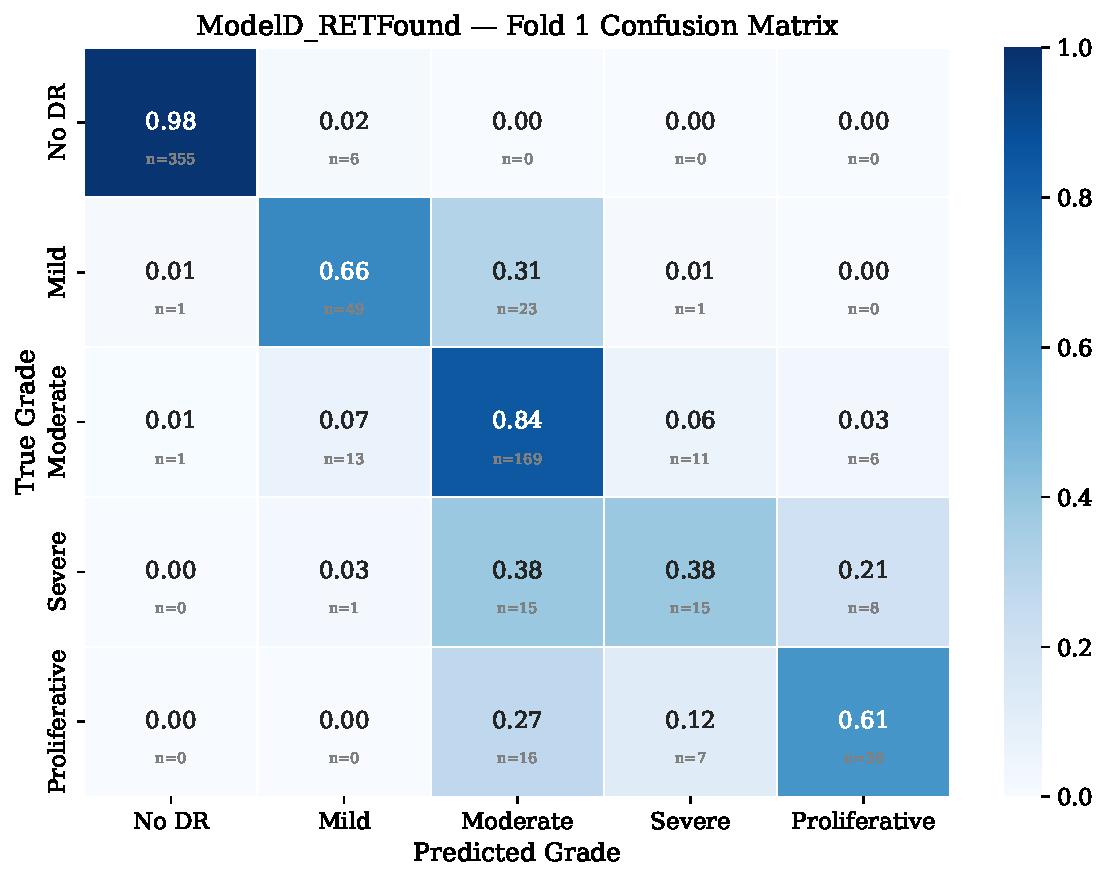
\includegraphics[width=\textwidth]{modelD_fold1_cm.pdf}
        \caption{RETFound + LoRA}
    \end{subfigure}
    \hfill
    \begin{subfigure}[b]{0.48\textwidth}
        \centering
        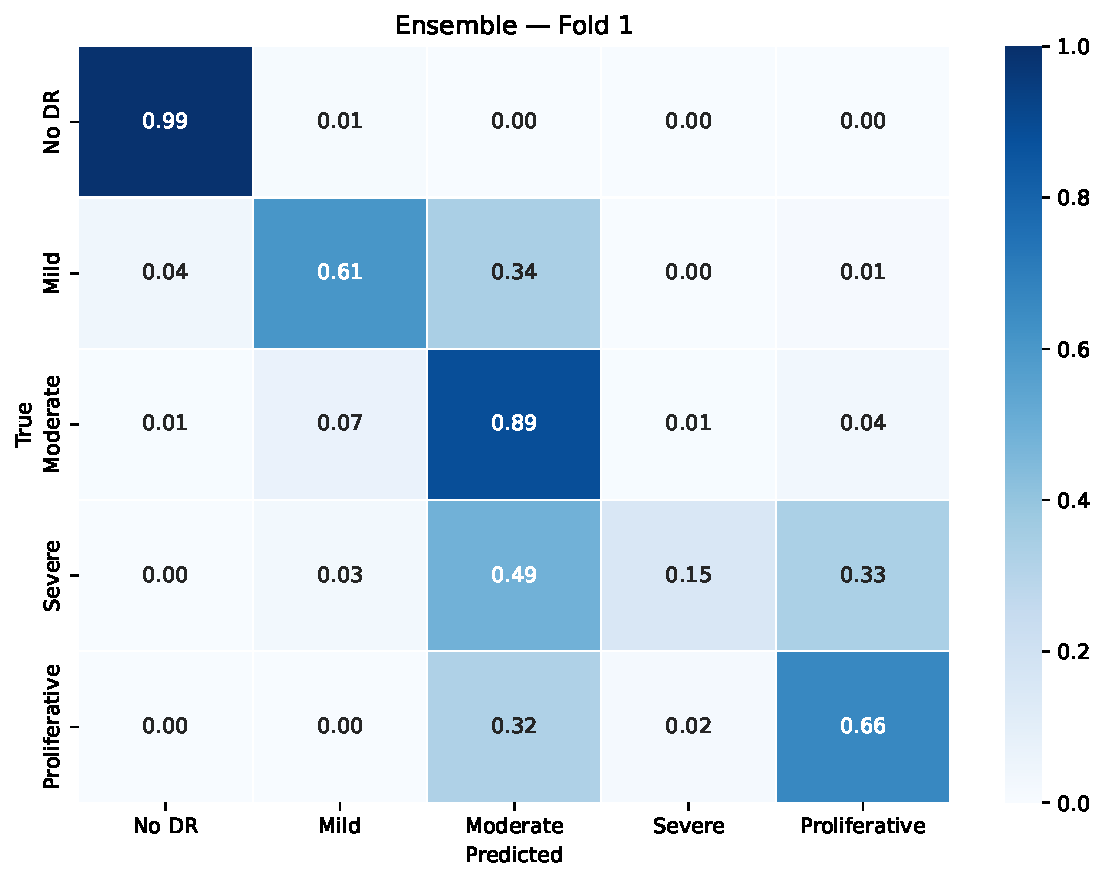
\includegraphics[width=\textwidth]{ensemble_fold1_cm.pdf}
        \caption{Ensemble}
    \end{subfigure}
    \caption{Normalised confusion matrices for Fold~1. Rows represent true grades, columns represent predicted grades. Values indicate the proportion of samples in each true class assigned to each predicted class.}
    \label{fig:confusion_matrices}
\end{figure}

Across all models and folds, the confusion matrices exhibit consistent patterns:

\begin{enumerate}
    \item \textbf{Grade 0 (No DR) is classified most accurately}, with recall typically exceeding 90\%. This is expected given the large representation of Grade~0 in the training set and the distinctiveness of a healthy fundus.
    
    \item \textbf{Grade 1 (Mild NPDR) is the most frequently misclassified grade}, with substantial confusion between Grades~0 and~2. This reflects the clinical reality that mild NPDR---characterised by a small number of microaneurysms---is the most subtle and subjective grade to distinguish.
    
    \item \textbf{Grade 4 (Proliferative DR) achieves high recall} despite being a minority class, likely because proliferative changes (neovascularisation, vitreous haemorrhage) produce visually dramatic pathology that is readily distinguishable.
    
    \item \textbf{Misclassifications are predominantly between adjacent grades.} The ordinal regression framework successfully minimises distant misclassifications (e.g., Grade~0 misclassified as Grade~4), which would be clinically dangerous. This is a direct consequence of the CORN loss, which trains rank-consistent classifiers.
\end{enumerate}

\section{ROC and Precision-Recall Analysis}
\label{sec:roc_pr}

The One-vs-Rest (OvR) ROC and Precision-Recall curves, generated for each fold and model, confirm the discriminative ability of the CORN-based probability estimates. Figure~\ref{fig:roc_curves} shows the ROC curves for all three models on Fold~1.

\begin{figure}[htbp]
    \centering
    \begin{subfigure}[b]{0.32\textwidth}
        \centering
        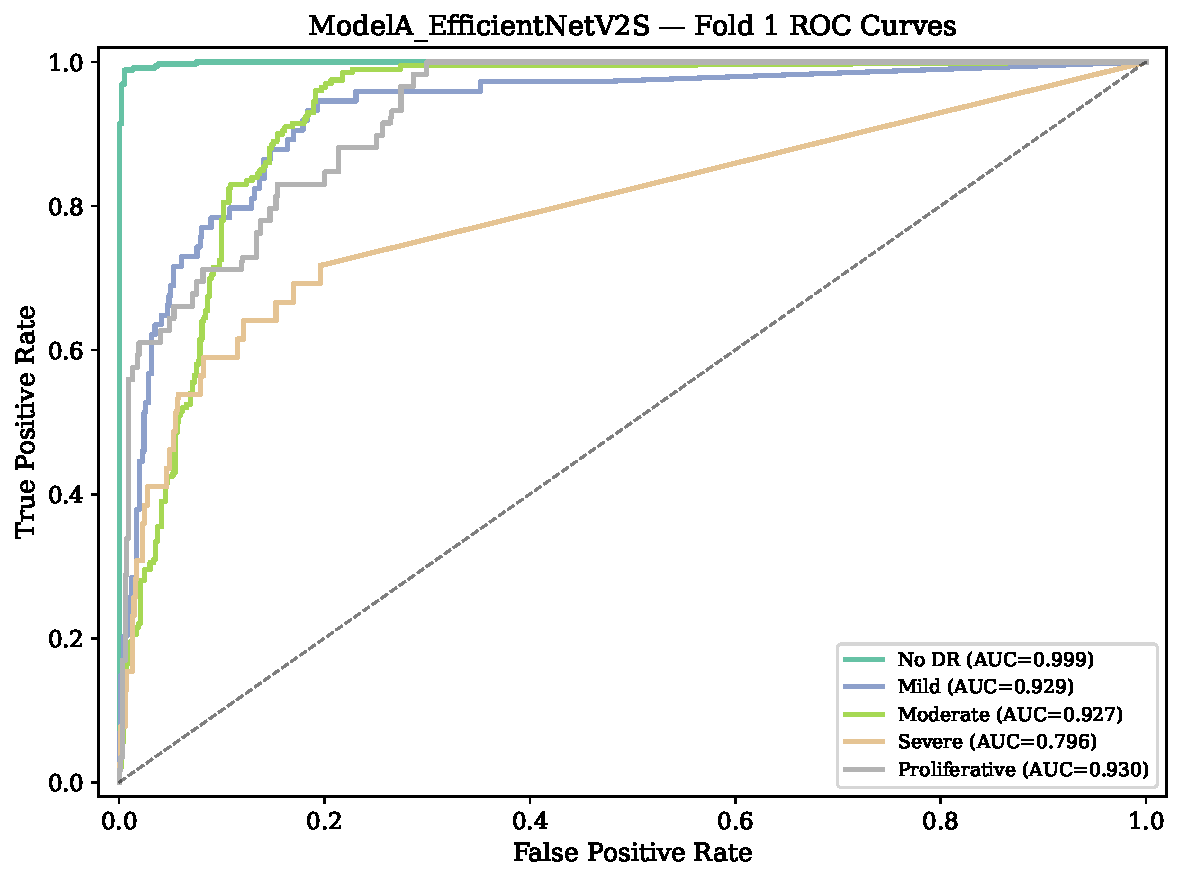
\includegraphics[width=\textwidth]{modelA_fold1_roc.pdf}
        \caption{EfficientNetV2-S}
    \end{subfigure}
    \hfill
    \begin{subfigure}[b]{0.32\textwidth}
        \centering
        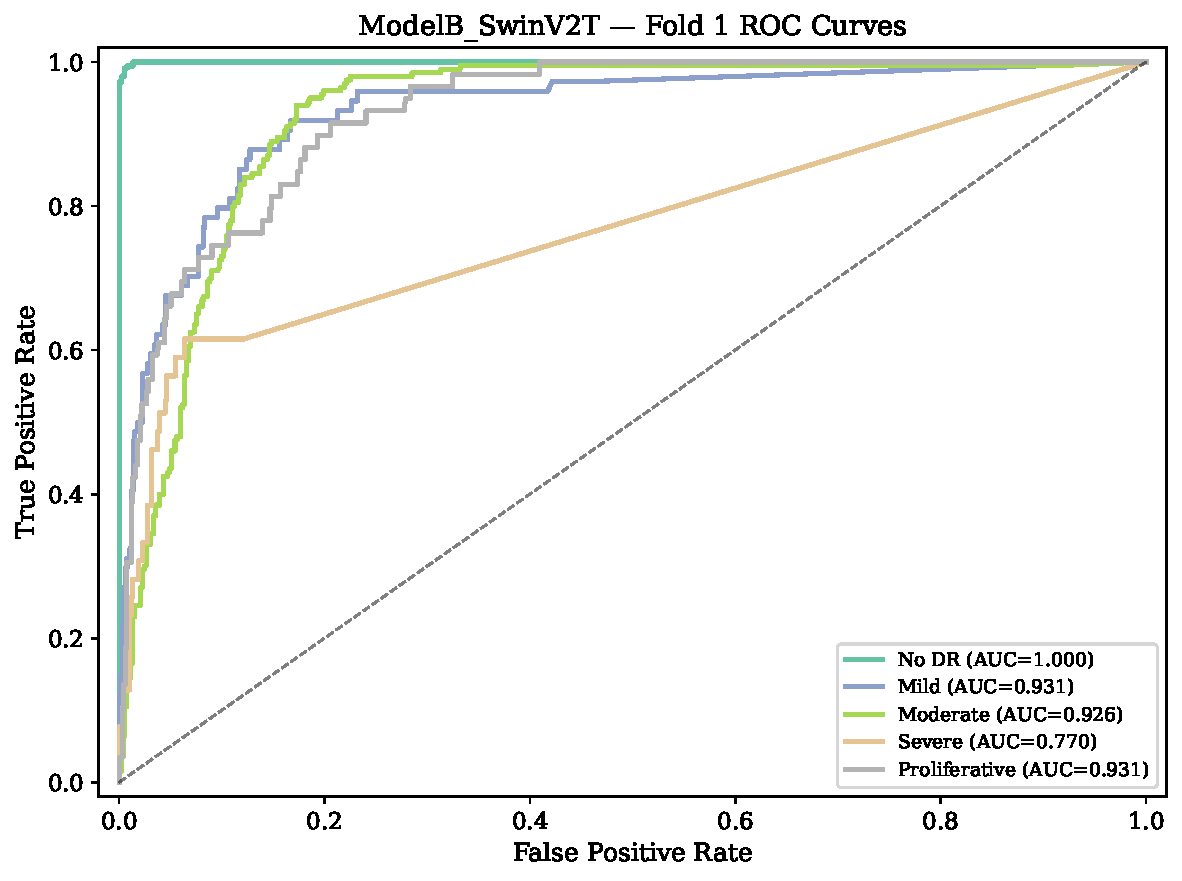
\includegraphics[width=\textwidth]{modelB_fold1_roc.pdf}
        \caption{Swin-V2-Tiny}
    \end{subfigure}
    \hfill
    \begin{subfigure}[b]{0.32\textwidth}
        \centering
        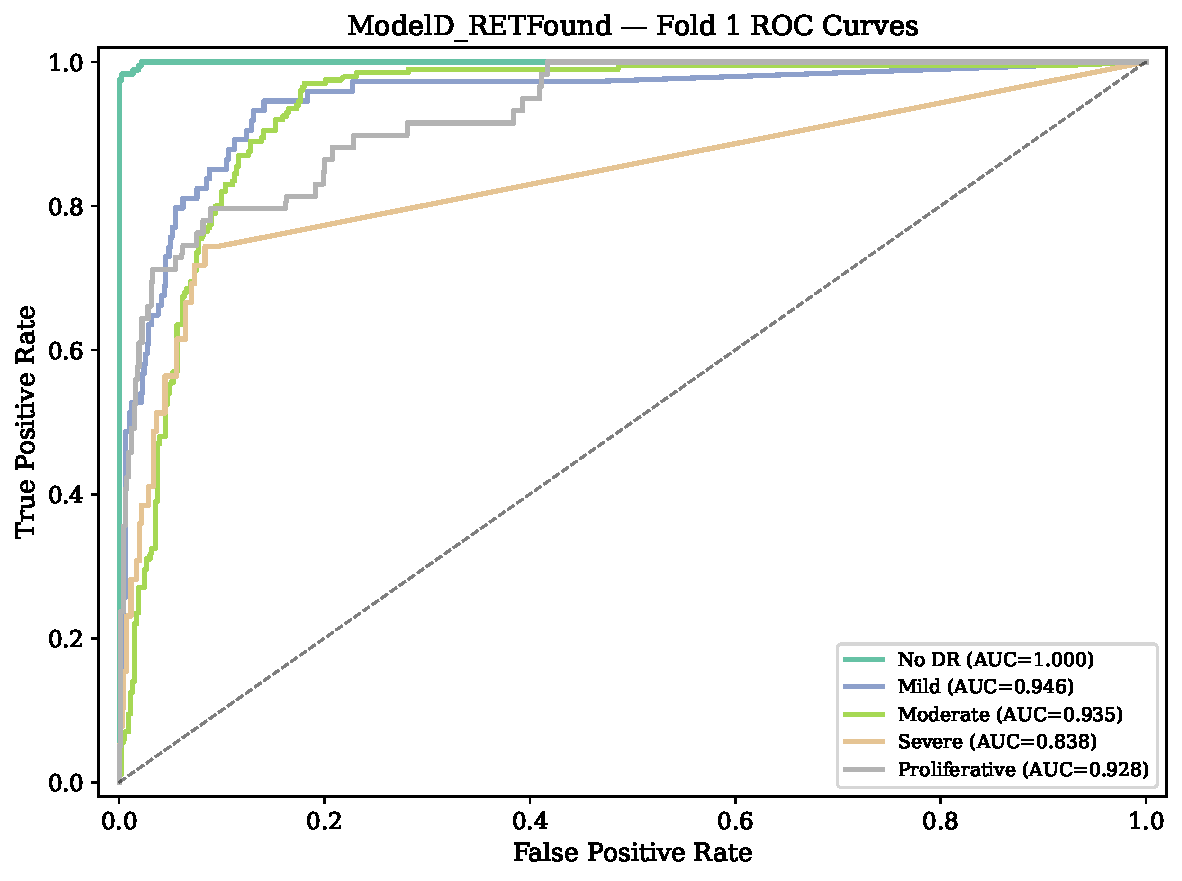
\includegraphics[width=\textwidth]{modelD_fold1_roc.pdf}
        \caption{RETFound + LoRA}
    \end{subfigure}
    \caption{ROC curves (One-vs-Rest) for Fold~1. Each curve represents the binary discrimination between one DR grade and all others. Per-class AUC values are shown in the legends.}
    \label{fig:roc_curves}
\end{figure}

\begin{figure}[htbp]
    \centering
    \begin{subfigure}[b]{0.32\textwidth}
        \centering
        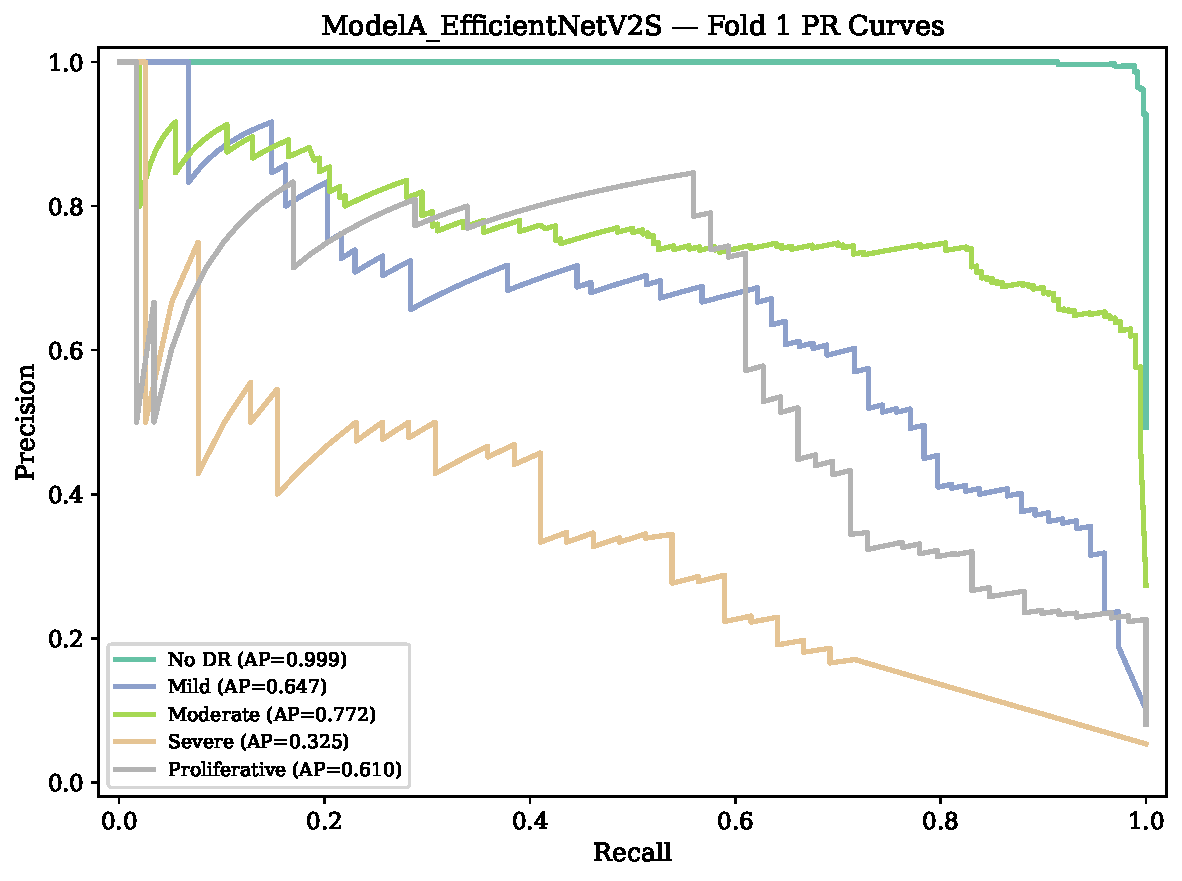
\includegraphics[width=\textwidth]{modelA_fold1_pr.pdf}
        \caption{EfficientNetV2-S}
    \end{subfigure}
    \hfill
    \begin{subfigure}[b]{0.32\textwidth}
        \centering
        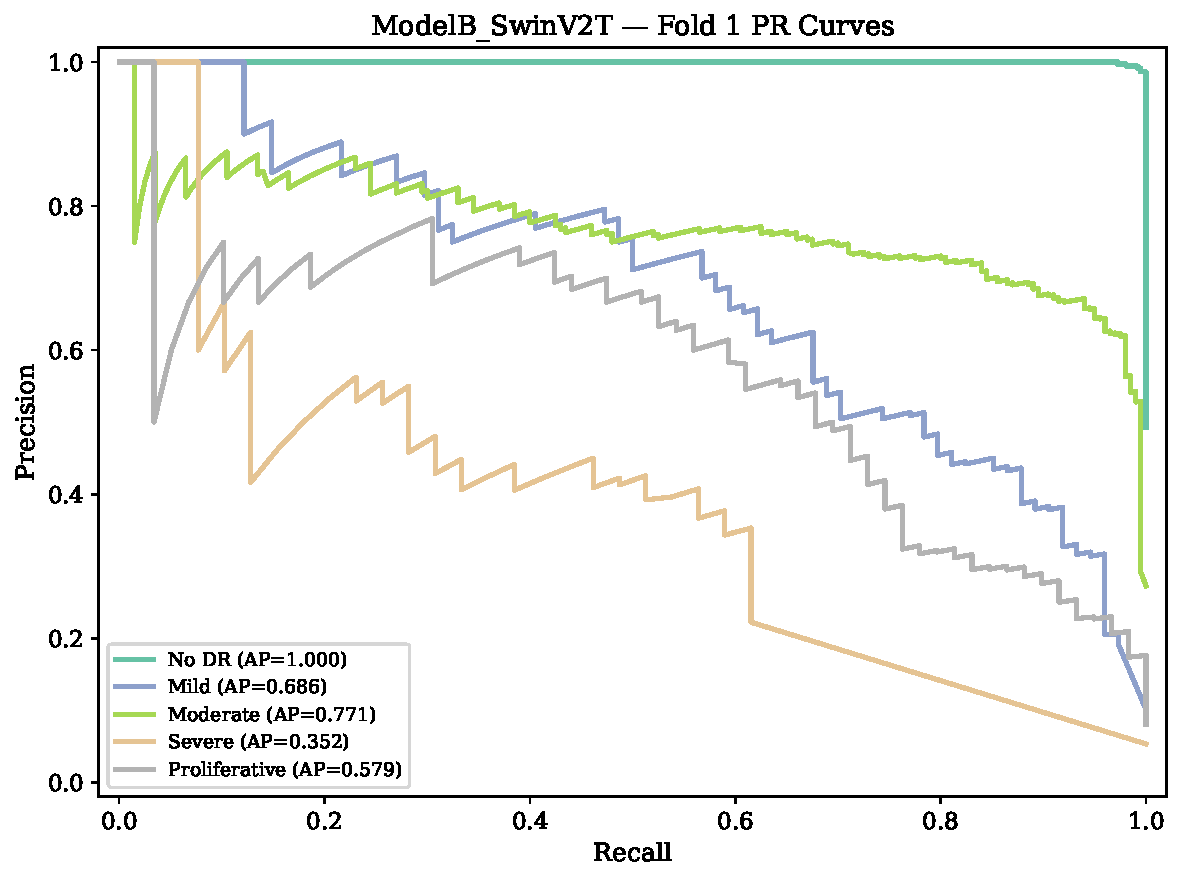
\includegraphics[width=\textwidth]{modelB_fold1_pr.pdf}
        \caption{Swin-V2-Tiny}
    \end{subfigure}
    \hfill
    \begin{subfigure}[b]{0.32\textwidth}
        \centering
        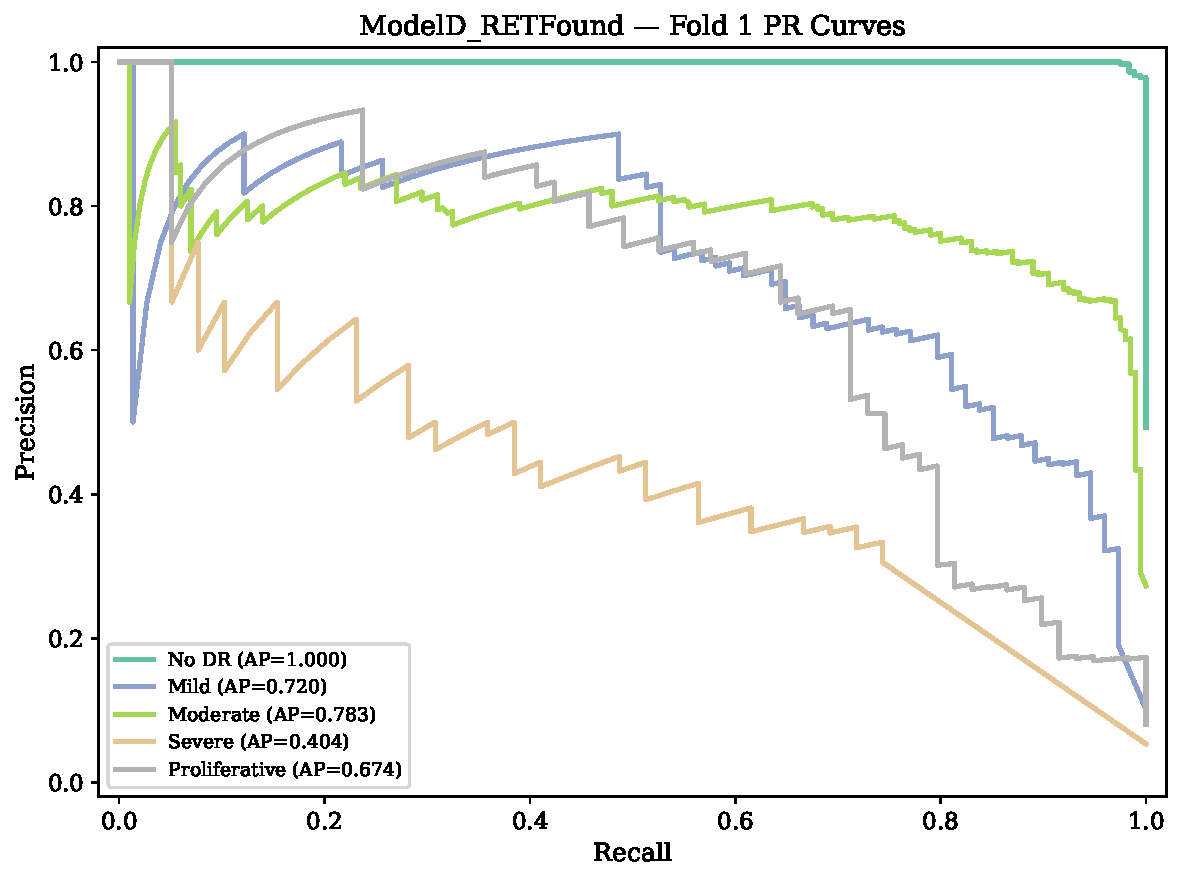
\includegraphics[width=\textwidth]{modelD_fold1_pr.pdf}
        \caption{RETFound + LoRA}
    \end{subfigure}
    \caption{Precision-Recall curves (One-vs-Rest) for Fold~1. Average precision (AP) values are shown in the legends for each DR grade.}
    \label{fig:pr_curves}
\end{figure}

Across all models, the per-class AUC values consistently exceed 0.90 for Grades~0, 3, and~4, with Grade~1 (Mild NPDR) exhibiting the lowest AUC (typically 0.85--0.90), consistent with the confusion matrix analysis. The Precision-Recall curves show similar trends, with Grade~1 and the minority classes (Grades~3 and~4) exhibiting lower average precision due to the class imbalance.

\section{Training Dynamics}
\label{sec:training_curves}

Figure~\ref{fig:training_curves} presents the training curves (loss, QWK, and learning rate) for EfficientNetV2-S and RETFound on Fold~1, illustrating the learning dynamics of each architecture.

\begin{figure}[htbp]
    \centering
    \begin{subfigure}[b]{0.48\textwidth}
        \centering
        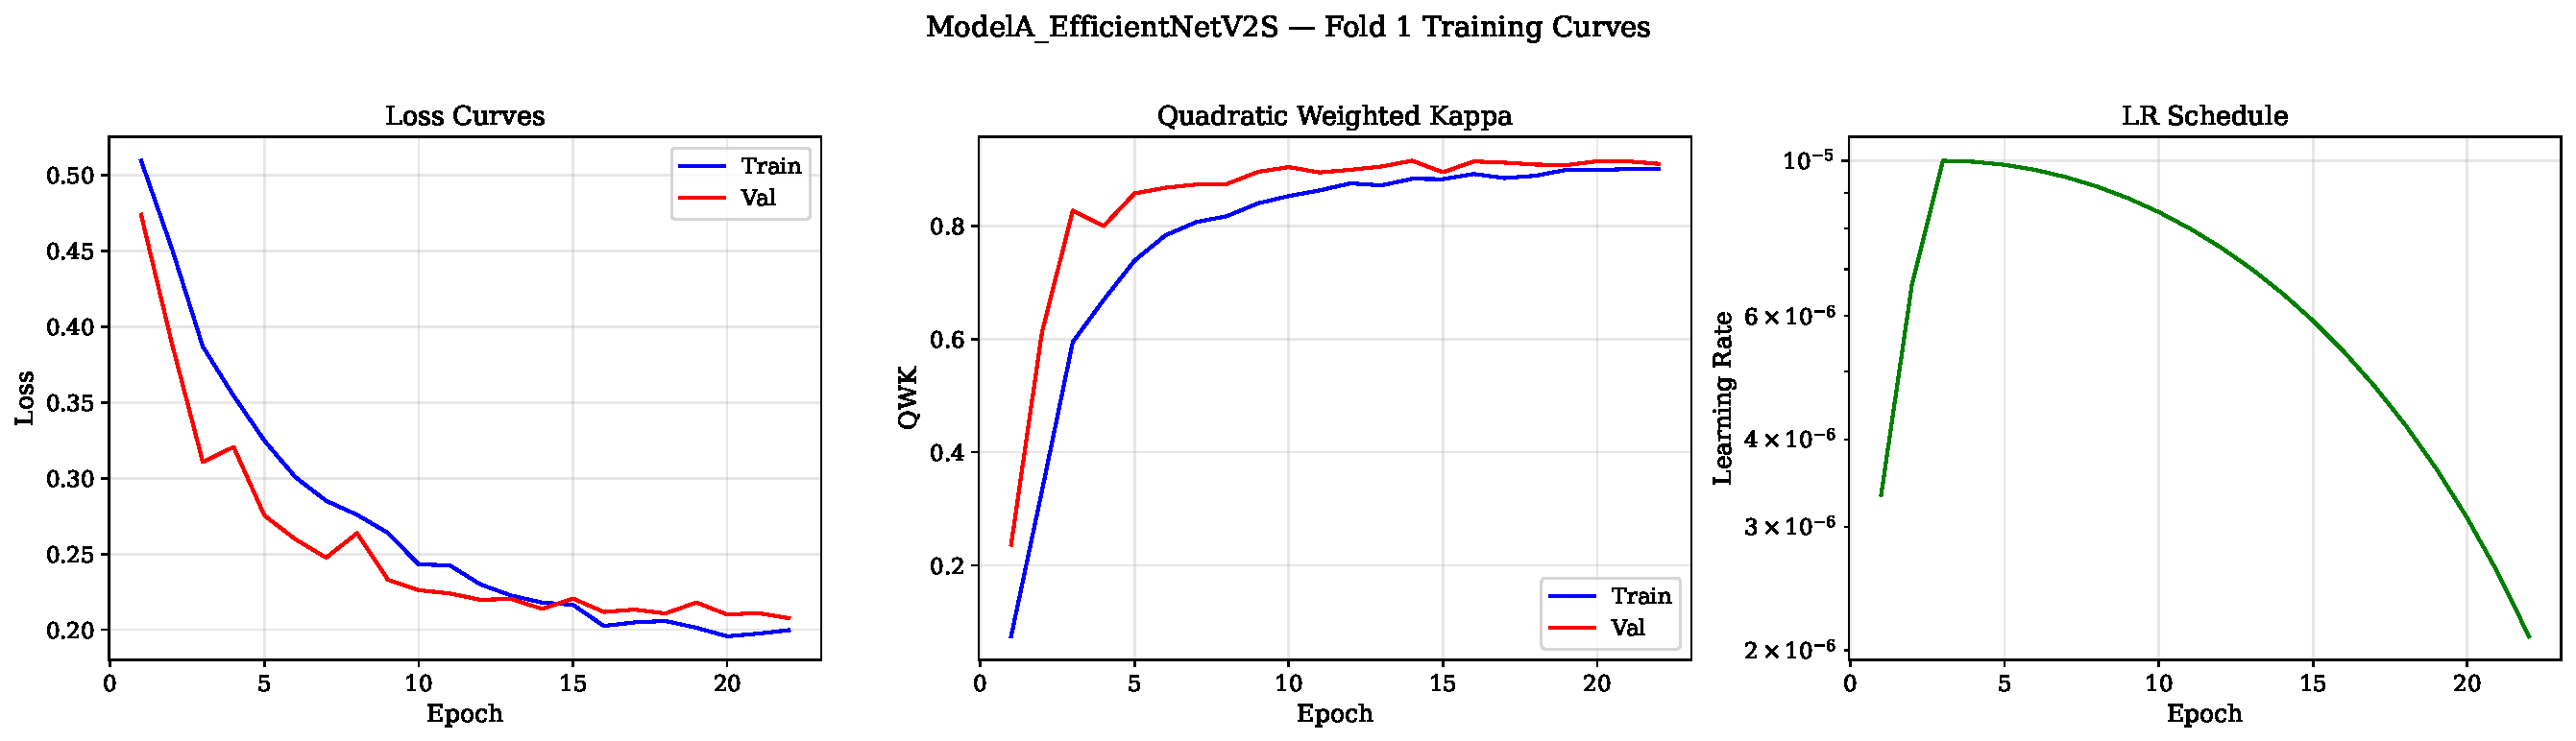
\includegraphics[width=\textwidth]{modelA_fold1_curves.pdf}
        \caption{EfficientNetV2-S}
    \end{subfigure}
    \hfill
    \begin{subfigure}[b]{0.48\textwidth}
        \centering
        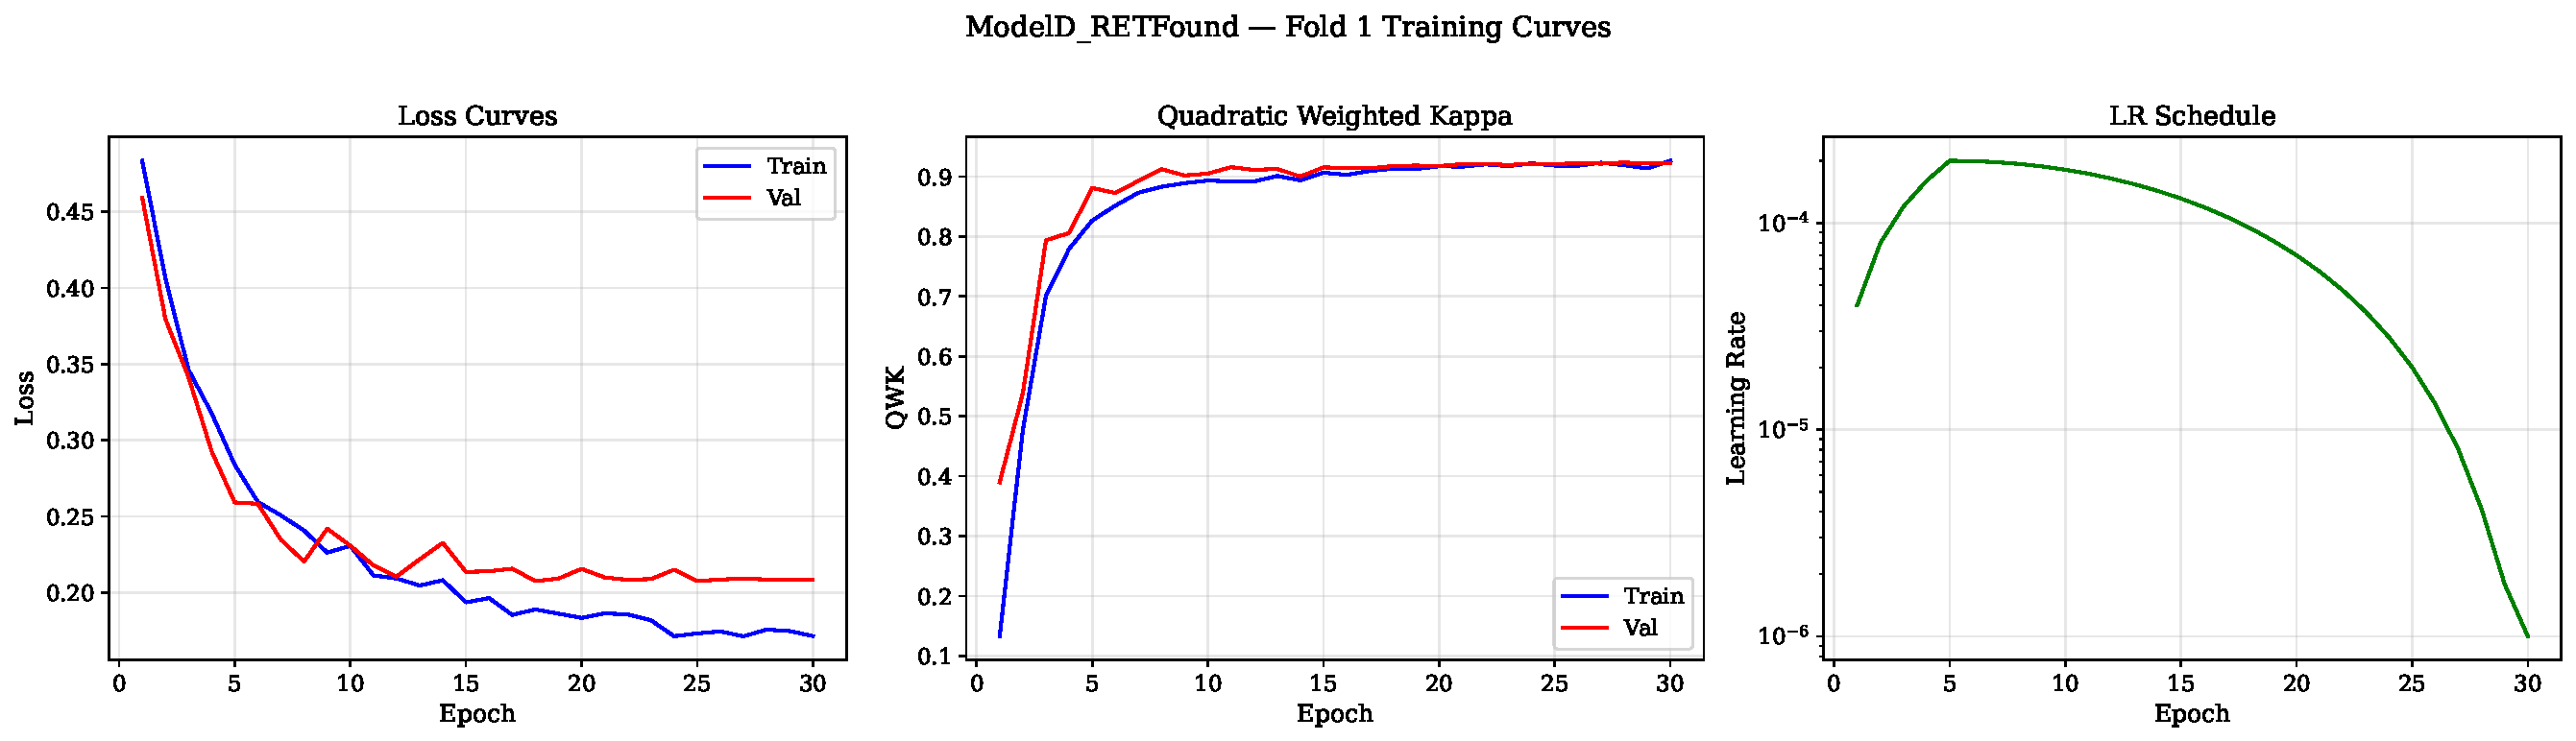
\includegraphics[width=\textwidth]{modelD_fold1_curves.pdf}
        \caption{RETFound + LoRA}
    \end{subfigure}
    \caption{Training curves for Fold~1 showing loss convergence, QWK progression, and learning rate schedule. The linear warmup phase is visible in the first few epochs, followed by cosine decay.}
    \label{fig:training_curves}
\end{figure}

\section{Latent Space Visualisation}
\label{sec:latent_space}

UMAP and t-SNE projections of the penultimate feature vectors provide qualitative insight into the learned representations. Figure~\ref{fig:umap} shows the UMAP projections for all three models on Fold~1.

\begin{figure}[htbp]
    \centering
    \begin{subfigure}[b]{0.32\textwidth}
        \centering
        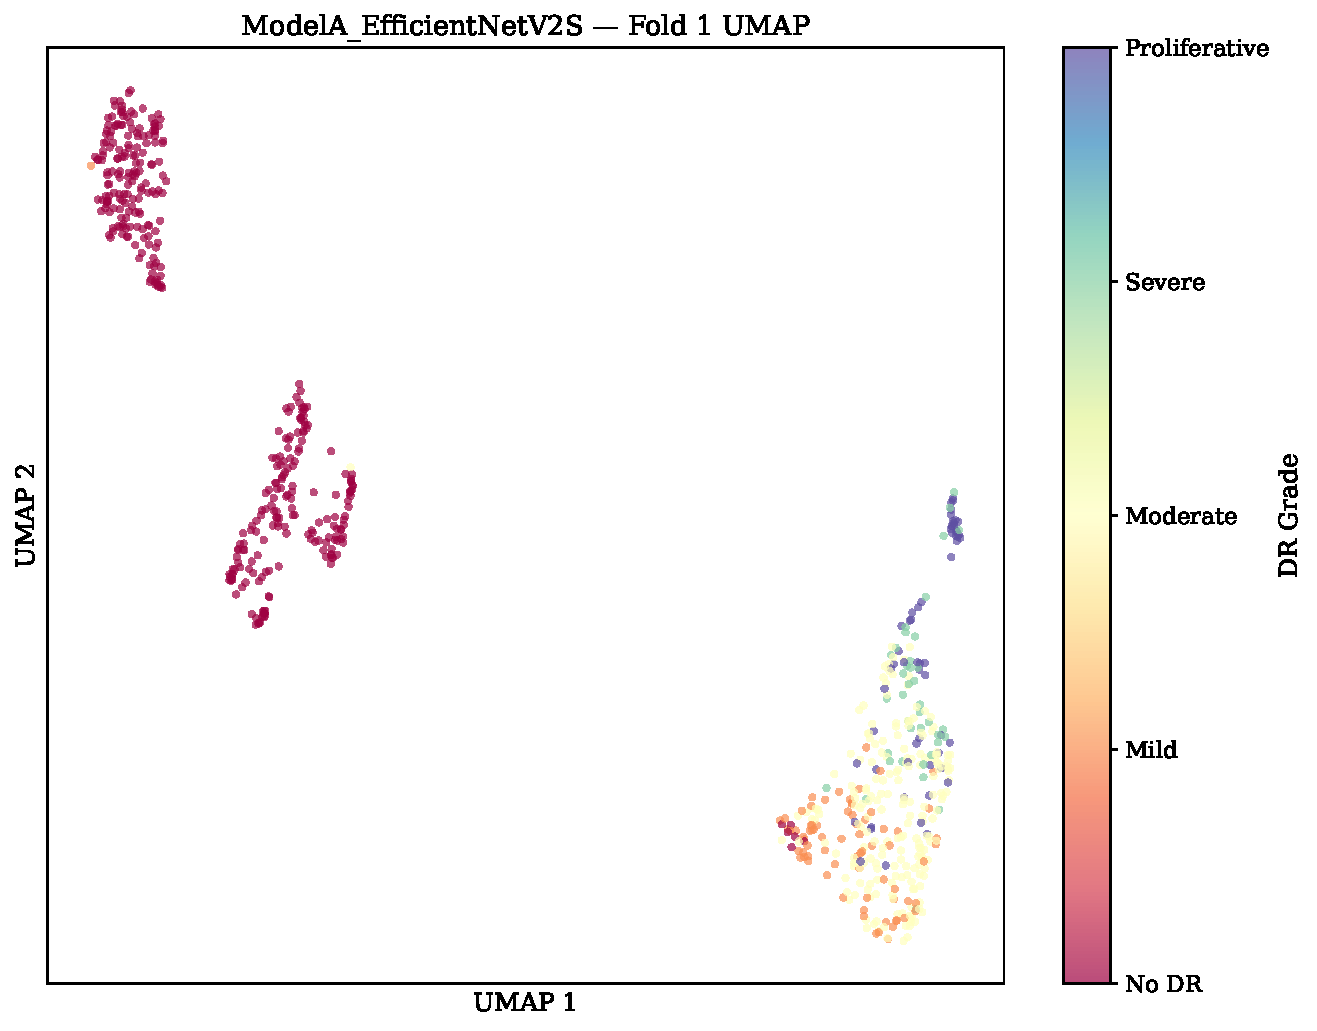
\includegraphics[width=\textwidth]{modelA_fold1_umap.pdf}
        \caption{EfficientNetV2-S}
    \end{subfigure}
    \hfill
    \begin{subfigure}[b]{0.32\textwidth}
        \centering
        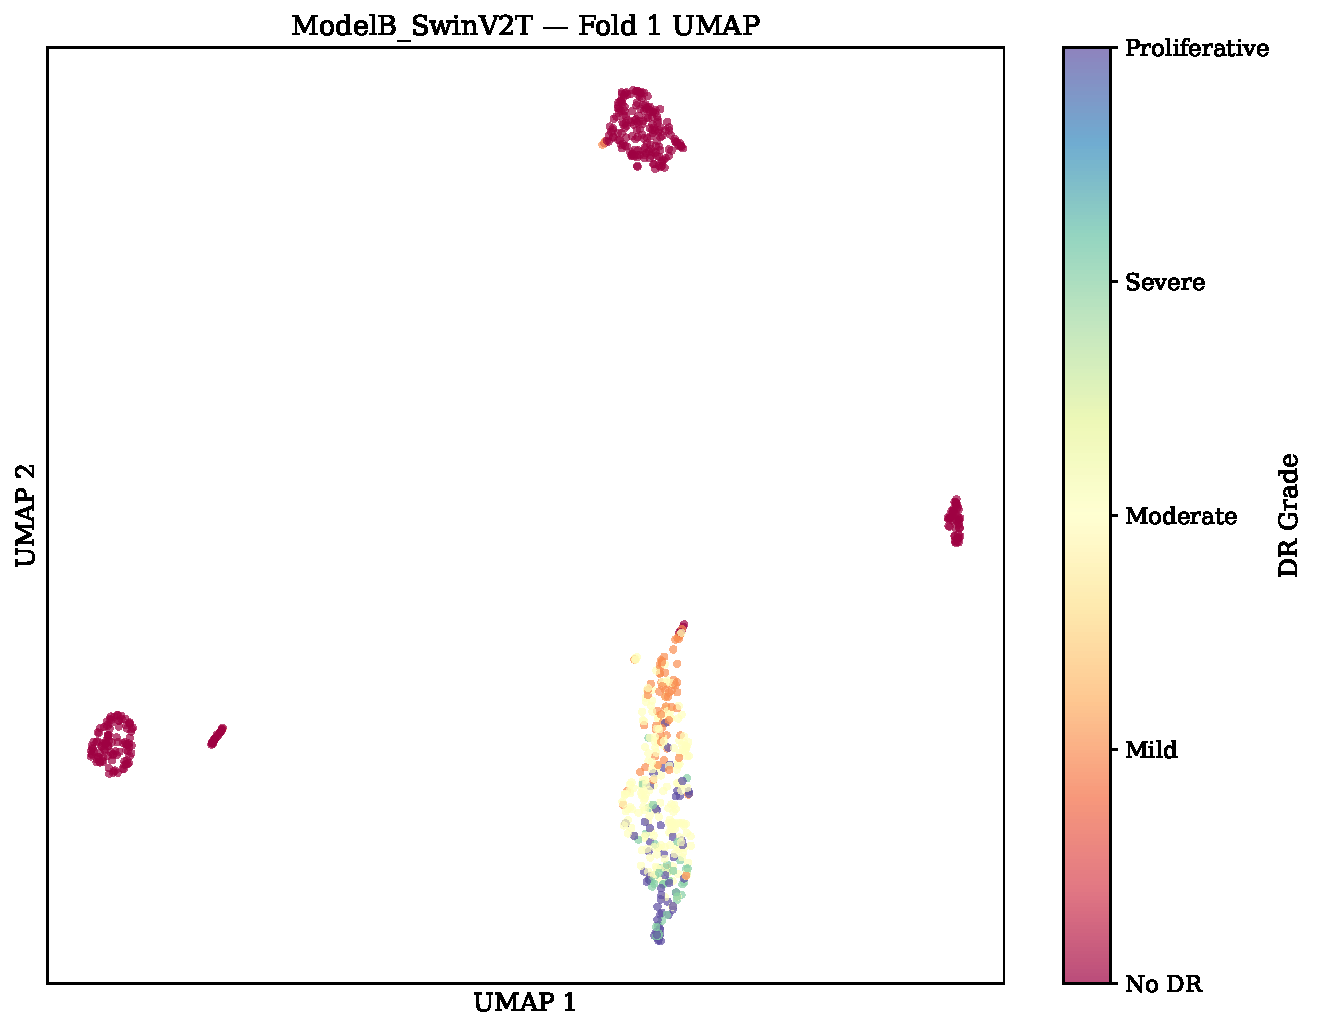
\includegraphics[width=\textwidth]{modelB_fold1_umap.pdf}
        \caption{Swin-V2-Tiny}
    \end{subfigure}
    \hfill
    \begin{subfigure}[b]{0.32\textwidth}
        \centering
        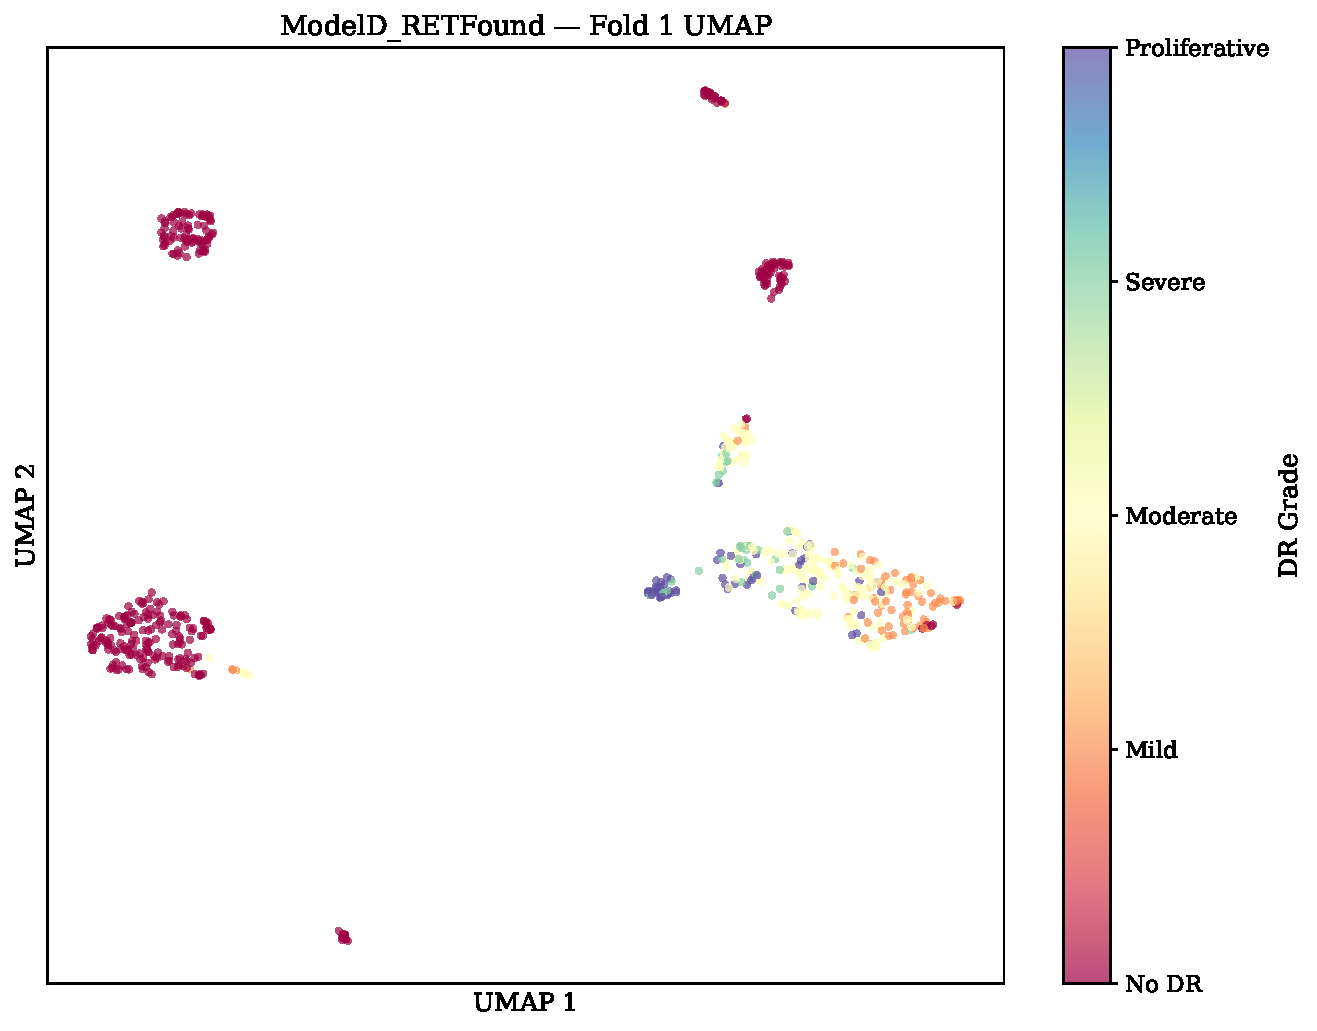
\includegraphics[width=\textwidth]{modelD_fold1_umap.pdf}
        \caption{RETFound + LoRA}
    \end{subfigure}
    \caption{UMAP projections of penultimate feature vectors for Fold~1, coloured by DR grade (0--4). Well-separated clusters indicate that the model has learned discriminative representations for each severity level.}
    \label{fig:umap}
\end{figure}

\begin{figure}[htbp]
    \centering
    \begin{subfigure}[b]{0.32\textwidth}
        \centering
        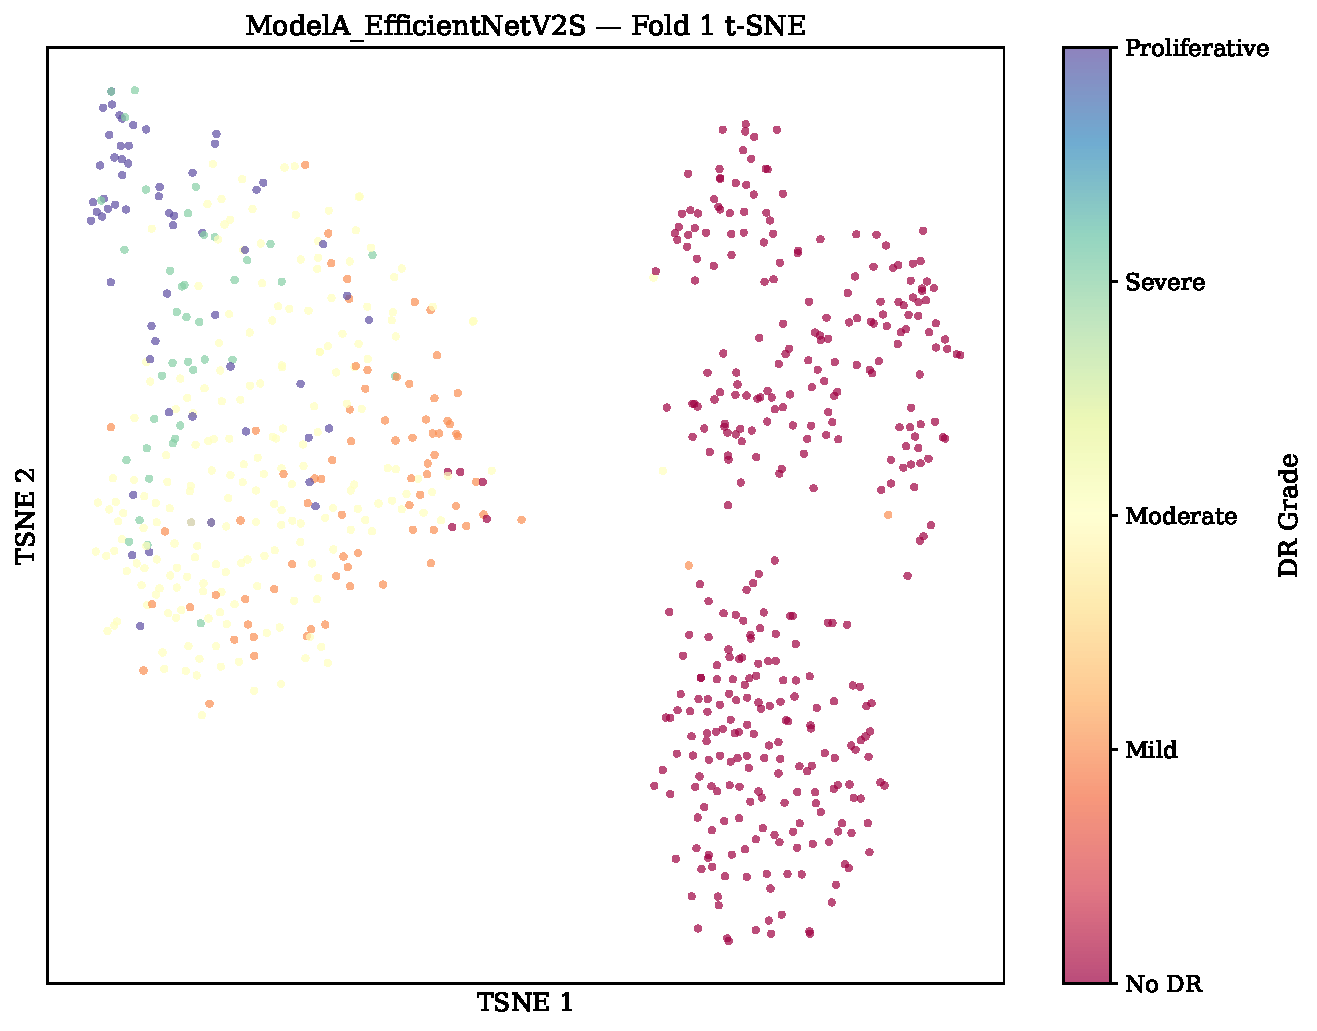
\includegraphics[width=\textwidth]{modelA_fold1_tsne.pdf}
        \caption{EfficientNetV2-S}
    \end{subfigure}
    \hfill
    \begin{subfigure}[b]{0.32\textwidth}
        \centering
        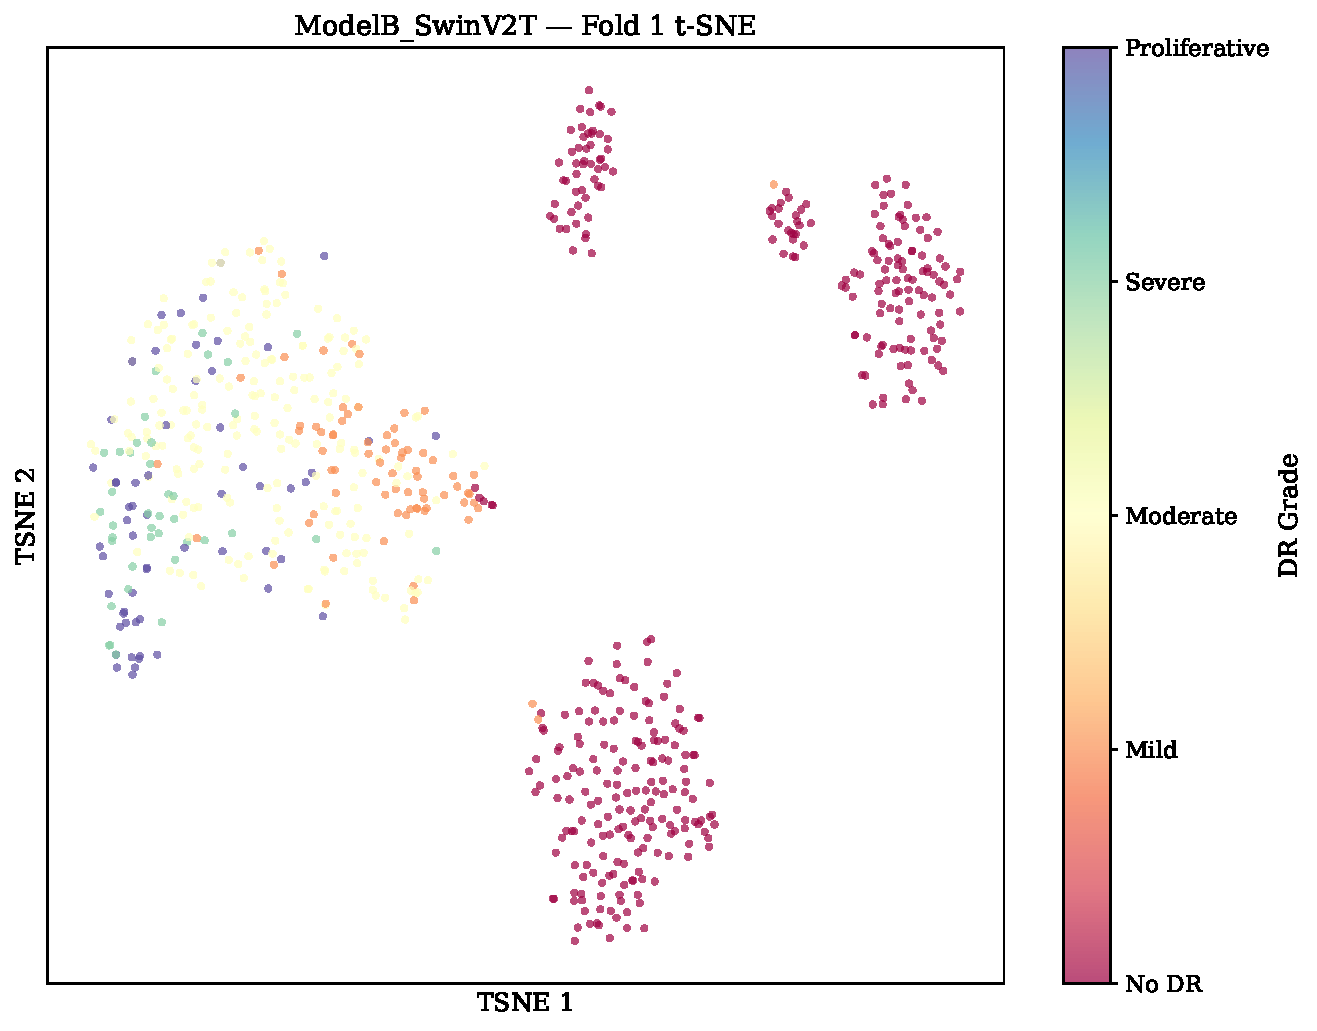
\includegraphics[width=\textwidth]{modelB_fold1_tsne.pdf}
        \caption{Swin-V2-Tiny}
    \end{subfigure}
    \hfill
    \begin{subfigure}[b]{0.32\textwidth}
        \centering
        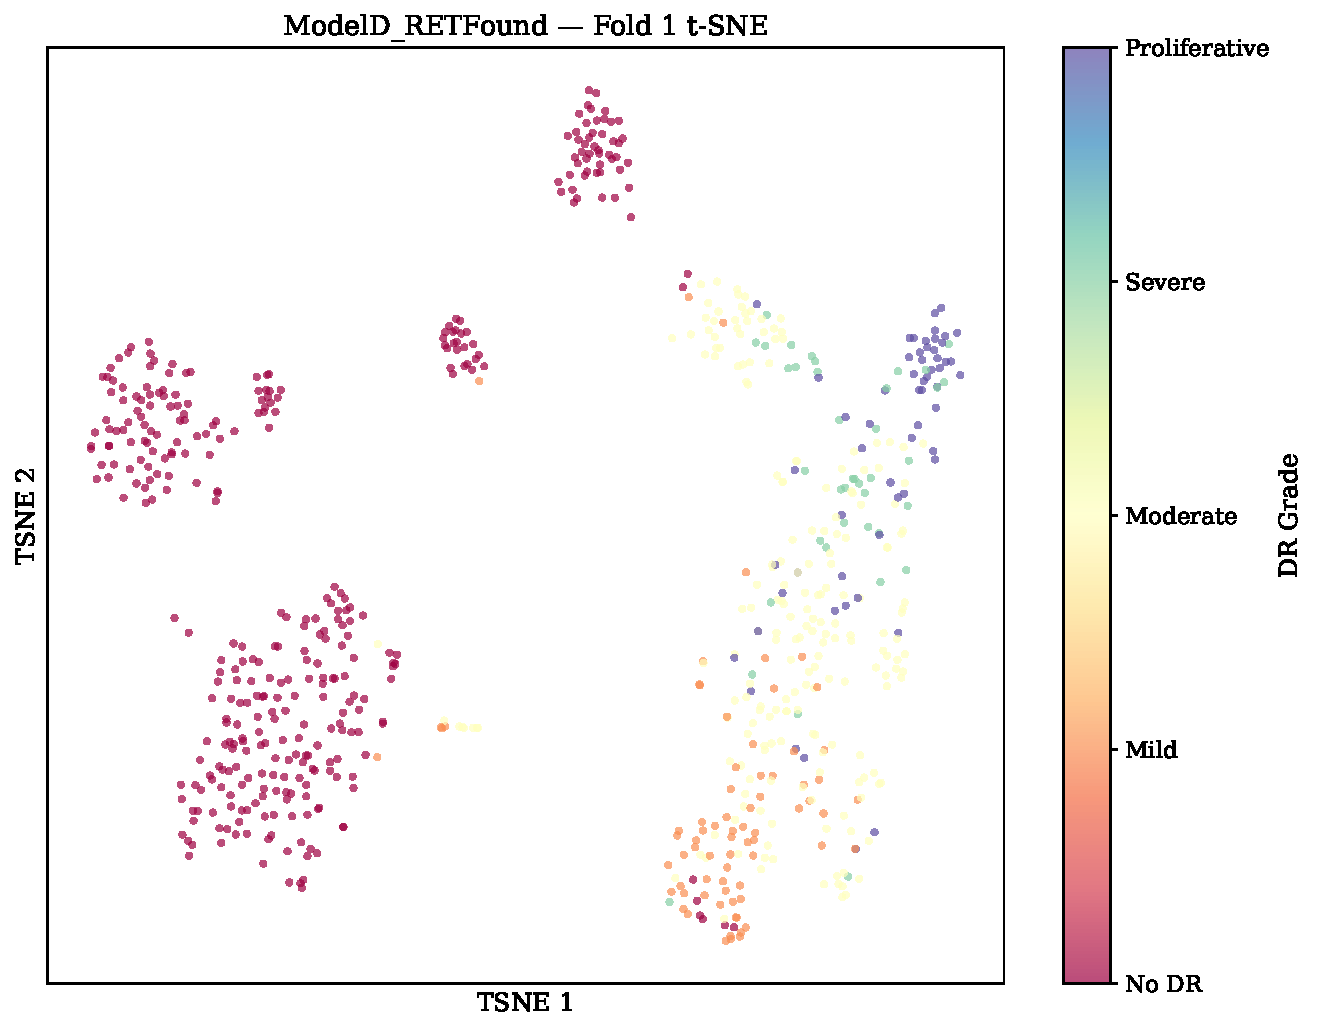
\includegraphics[width=\textwidth]{modelD_fold1_tsne.pdf}
        \caption{RETFound + LoRA}
    \end{subfigure}
    \caption{t-SNE projections of penultimate feature vectors for Fold~1, coloured by DR grade (0--4). The ordinal structure is visible as adjacent grades form neighbouring clusters.}
    \label{fig:tsne}
\end{figure}

The latent space visualisations reveal that:
\begin{itemize}
    \item All three models learn well-separated cluster structures corresponding to the five DR grades, confirming effective feature learning.
    \item RETFound produces the most compact and well-separated clusters, consistent with its superior classification performance.
    \item The overlap regions between clusters correspond to the adjacent-grade confusion observed in the confusion matrices, particularly between Grades~0/1 and Grades~1/2.
    \item The ordinal structure is preserved in the latent space: clusters corresponding to adjacent grades are spatially closer than those corresponding to distant grades, reflecting the ordinal nature of the CORN representation.
\end{itemize}

\section{Comparative Performance Charts}
\label{sec:comparative_charts}

Figure~\ref{fig:qwk_bar} presents a comparative bar chart of mean QWK scores, and Figure~\ref{fig:qwk_box} shows the stability analysis through box plots of QWK distributions across the five folds.

\begin{figure}[htbp]
    \centering
    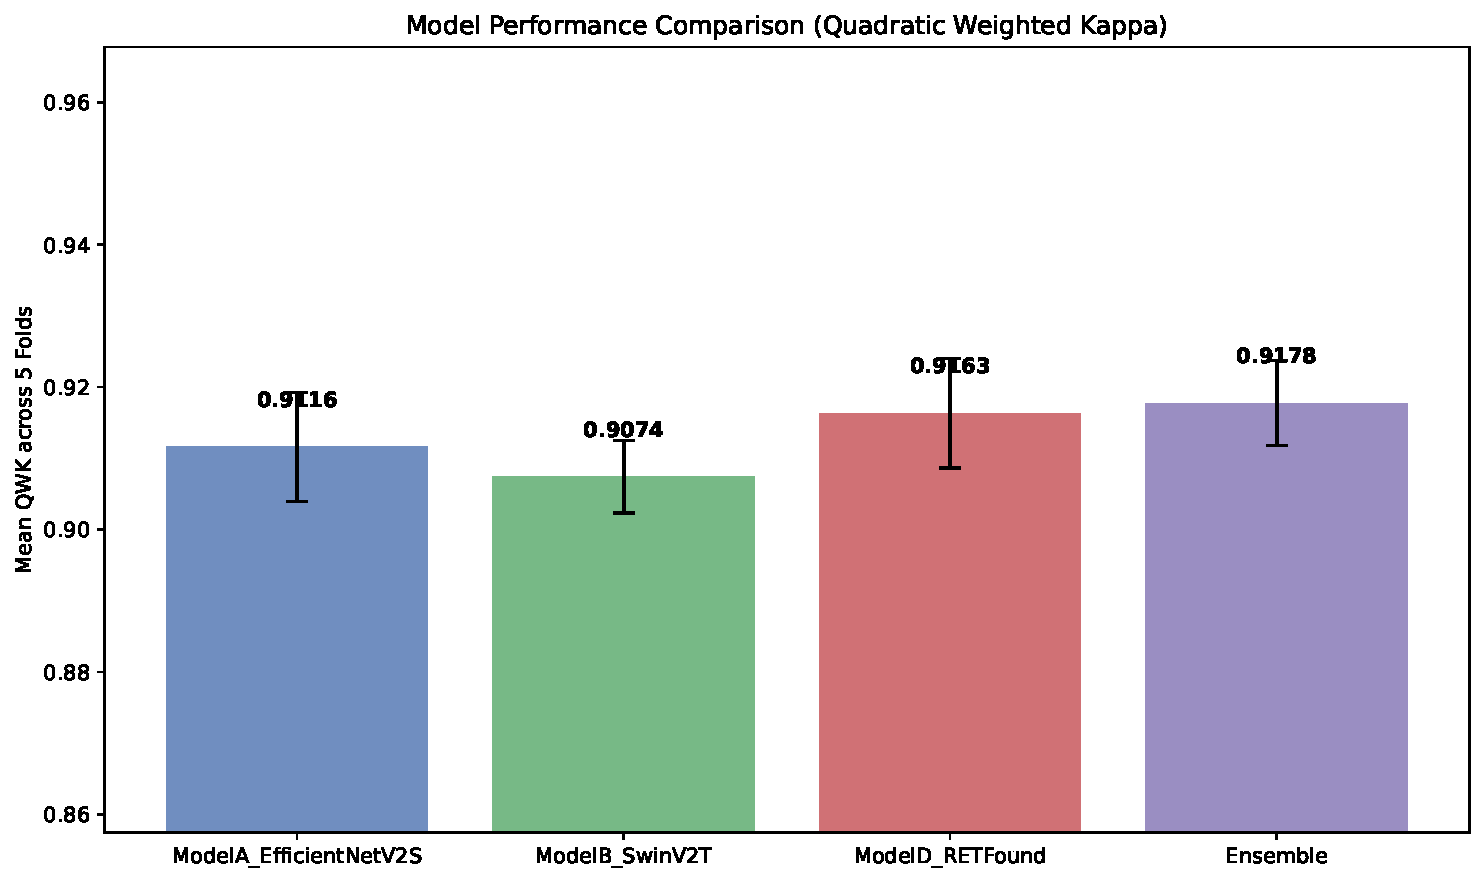
\includegraphics[width=0.75\textwidth]{comparative_qwk_bar.pdf}
    \caption{Comparative bar chart of mean QWK across 5-fold cross-validation for all models and the ensemble. Error bars represent $\pm 1$ standard deviation. The ensemble achieves the highest mean QWK.}
    \label{fig:qwk_bar}
\end{figure}

\begin{figure}[htbp]
    \centering
    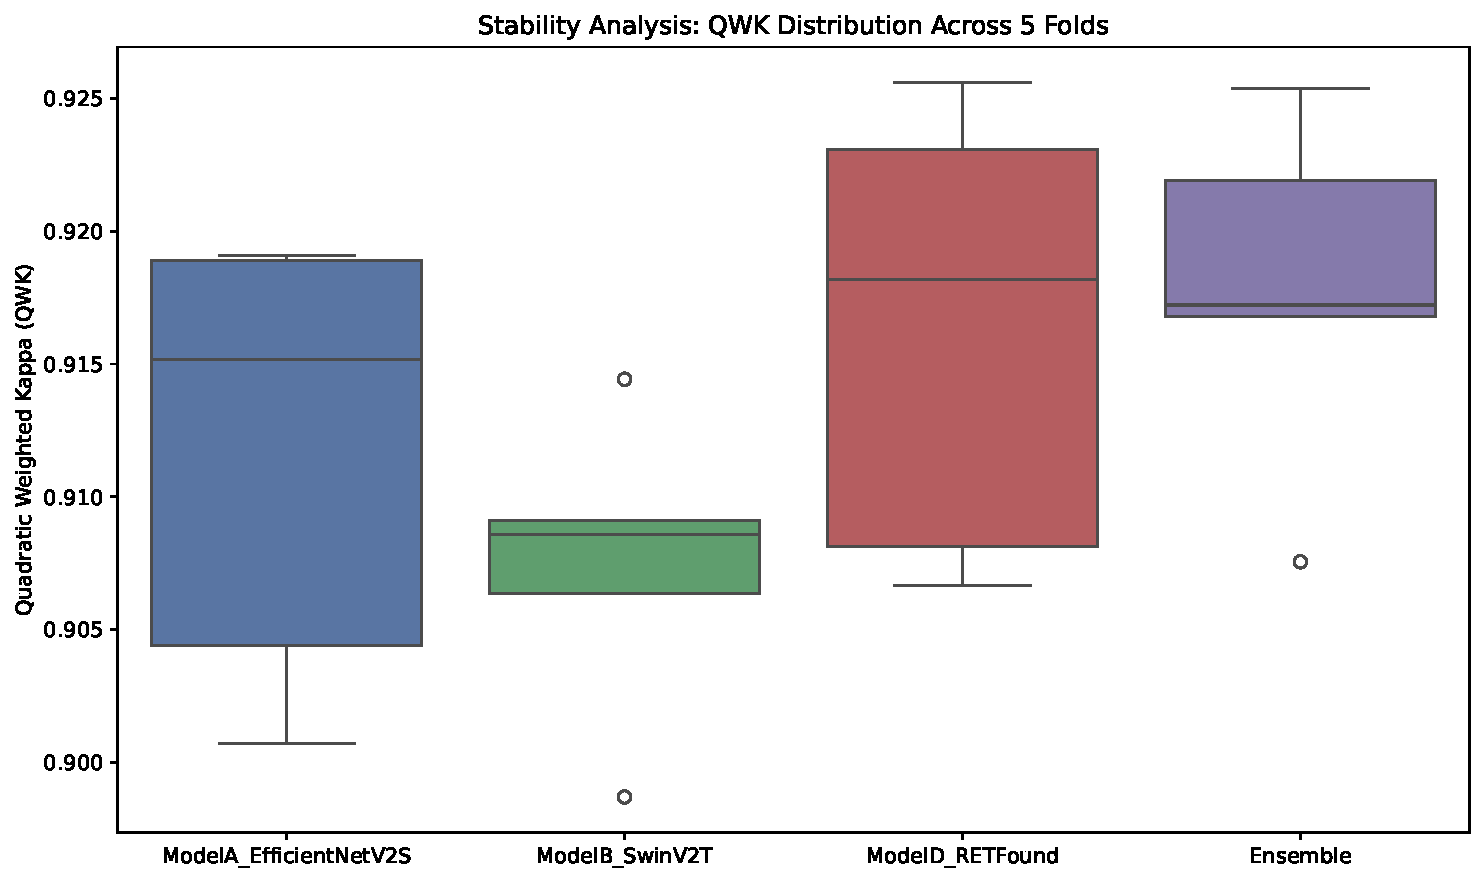
\includegraphics[width=0.75\textwidth]{comparative_qwk_box.pdf}
    \caption{Box plot showing the distribution of QWK scores across 5 folds for each model and the ensemble. Swin-V2-Tiny exhibits the narrowest interquartile range (most stable), while the ensemble combines high mean performance with reduced variance.}
    \label{fig:qwk_box}
\end{figure}

\section{Model Prediction Correlation}
\label{sec:correlation}

To assess the diversity of the three models' predictions---a prerequisite for effective ensemble fusion---we compute the pairwise Spearman rank correlation between model predictions on the Fold~1 validation set (Figure~\ref{fig:correlation}).

\begin{figure}[htbp]
    \centering
    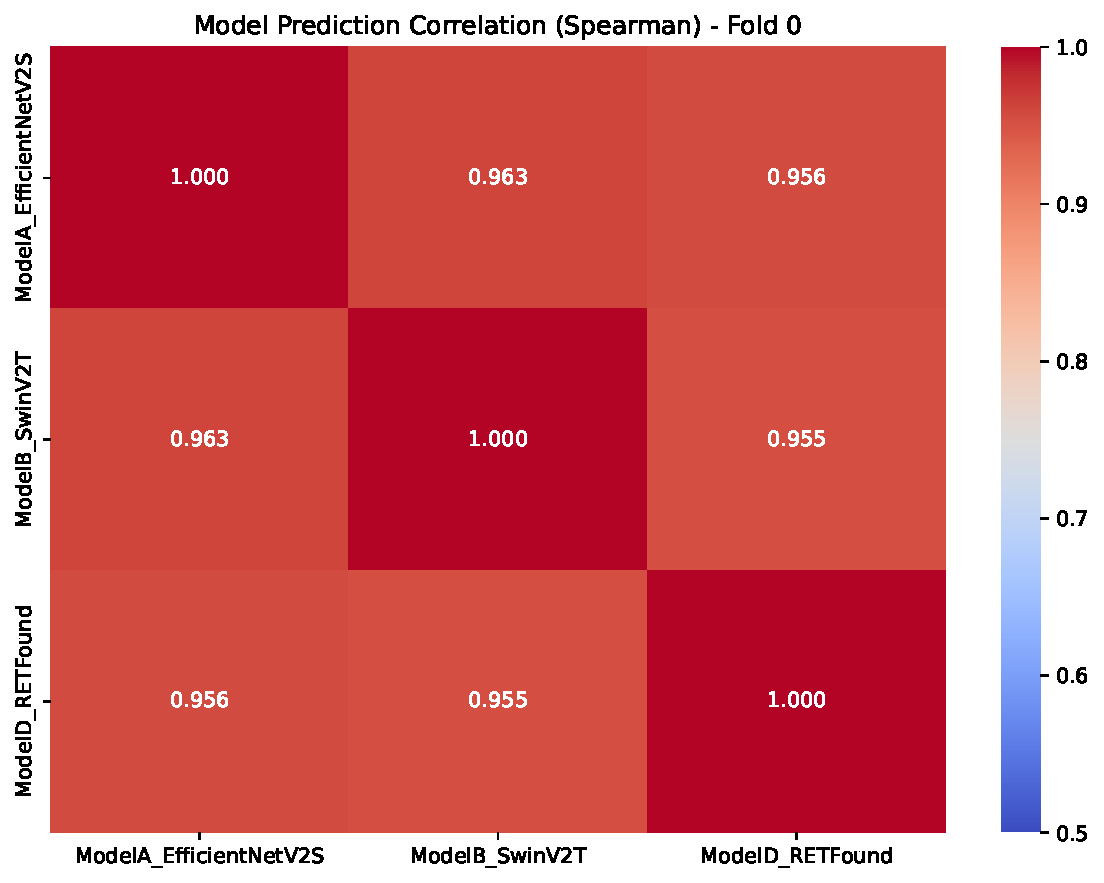
\includegraphics[width=0.6\textwidth]{model_correlation_heatmap.pdf}
    \caption{Spearman rank correlation matrix between the predictions of the three models on Fold~1. Lower correlation indicates greater prediction diversity, which benefits ensemble fusion. RETFound shows the lowest average correlation with the other models.}
    \label{fig:correlation}
\end{figure}

The correlation analysis reveals moderate-to-high correlation between the models (typically $\rho = 0.85$--$0.92$), with RETFound showing the lowest average correlation with the other two models. This lower correlation confirms that the foundation model's representations, learned from domain-specific pretraining, capture aspects of retinal pathology that are distinct from those learned by ImageNet-pretrained CNN and transformer architectures. This diversity is precisely what enables the ensemble to improve upon the best individual model.

\section{Ablation Study}
\label{sec:model_c}

An additional architecture, designated Model~C, was initially explored as a CNN--Transformer hybrid that combined a CNN backbone for local feature extraction with a Transformer encoder for global reasoning. However, this architecture exhibited severe training stagnation during fine-tuning on the APTOS dataset, with QWK remaining near zero despite extensive hyperparameter search. The failure was attributed to the difficulty of simultaneously training randomly initialised Transformer layers and pretrained CNN backbone under the same learning rate, leading to catastrophic destruction of the pretrained features before the Transformer layers could converge. While differential learning rates partially mitigated this issue, the hybrid model's performance remained substantially below the other three architectures, and it was excluded from the final comparative analysis. This negative result underscores the challenges of training hybrid architectures on small datasets without careful stage-wise training protocols.

\chapter{Discussion}
\label{ch:discussion}

This chapter synthesises the experimental findings, analyses the trade-offs between the three architectural paradigms, examines the clinical implications of the proposed framework, and acknowledges its limitations.

\section{CNN vs.\ Transformer vs.\ Foundation Model}
\label{sec:arch_comparison}

The results of this ablation study provide empirical insight into the relative merits of the three dominant paradigms in modern computer vision when applied to medical image classification on a small, class-imbalanced dataset.

\subsection{EfficientNetV2-S: The Efficiency of Inductive Bias}

EfficientNetV2-S achieves strong performance ($\kappa = 0.9116$) with the fastest training time ($\sim$11 hours) and a moderate parameter count ($\sim$21M). Its success on the APTOS dataset can be attributed to the CNN's strong inductive biases---locality and translation equivariance---which are particularly advantageous when training data is limited. The convolutional filters are inherently suited to detecting the local textural patterns characteristic of DR lesions: microaneurysms, dot haemorrhages, and hard exudates are all spatially compact features that a CNN can learn from relatively few examples.

The Fused-MBConv blocks in the early stages provide efficient feature extraction, while the SE attention mechanism enables the network to selectively amplify informative channels. However, the purely local receptive field limits the model's ability to reason about global spatial relationships, such as the distribution of lesions across retinal quadrants---a criterion explicitly used in the clinical grading of Severe NPDR.

\subsection{Swin-V2-Tiny: Global Reasoning at a Cost}

Swin-V2-Tiny achieves the lowest mean QWK ($\kappa = 0.9074$) among the three models, though with the lowest variance ($\pm 0.0051$). This seemingly paradoxical result---better stability but worse mean performance---reflects the fundamental trade-off of transformer architectures on small datasets. The shifted-window self-attention mechanism provides the capacity for global spatial reasoning, but this flexibility comes at the cost of requiring more data to learn effective attention patterns. The stronger regularisation (weight decay $0.05$, dropout $0.20$) necessary to prevent overfitting on $\sim$2,930 training images per fold constrains the model's effective capacity, resulting in a performance ceiling below that of the CNN.

Nevertheless, the model's stable performance across folds ($\pm 0.0051$, the lowest variance) suggests that the transformer's attention mechanism, once learned, generalises robustly across different data partitions. This stability is valuable in clinical deployment, where consistent performance across patient populations is as important as peak accuracy.

\subsection{RETFound + LoRA: The Foundation Model Advantage}

RETFound achieves the highest individual QWK ($\kappa = 0.9163$) while training only 0.4\% of its parameters, representing a fundamentally different approach to the accuracy-efficiency trade-off. The model's strong performance can be attributed to two factors:

First, the MAE pretraining on 1.6 million retinal images has endowed the backbone with rich, domain-specific representations of retinal morphology. The frozen backbone already ``understands'' the visual language of fundus images---vascular branching patterns, optic disc structure, macular anatomy---without requiring any task-specific training on these features. This domain-specific initialisation provides a substantial advantage over ImageNet pretraining, where the network must repurpose features learned from natural images (e.g., textures of animals, objects) for the very different domain of retinal pathology.

Second, the LoRA adaptation strategy enables highly targeted fine-tuning of the attention mechanism's routing behaviour (through the QKV and output projections) without perturbing the feature representations learned during pretraining. The low-rank constraint ($r = 8$) acts as an implicit regulariser, preventing the small APTOS dataset from overwriting the pretrained representations.

The trade-off is computational: RETFound requires $\sim$11 hours of training despite having the fewest trainable parameters, due to the large forward pass through the 307M-parameter backbone (24 Transformer blocks at $224 \times 224$ resolution) and the overhead of gradient checkpointing.

\section{The Value of Ordinal Regression}
\label{sec:ordinal_value}

A central thesis of this work is that ordinal regression is superior to standard multi-class classification for disease severity grading. While a controlled experiment comparing CORN loss against cross-entropy loss is beyond the scope of this thesis, several indirect lines of evidence support this claim:

\begin{enumerate}
    \item \textbf{Confusion matrix structure:} The misclassification patterns in Figure~\ref{fig:confusion_matrices} are predominantly between adjacent grades, with virtually no distant misclassifications. This is a direct consequence of the rank-consistent predictions enforced by CORN.
    
    \item \textbf{High QWK relative to accuracy:} All models achieve QWK $> 0.90$ despite raw accuracy of only $\sim$82--84\%. This gap indicates that the few misclassifications that do occur are predominantly off-by-one errors, which incur minimal QWK penalty. Under standard cross-entropy (which does not encode ordinality), one would expect a higher proportion of distant misclassifications, resulting in lower QWK for similar accuracy levels.
    
    \item \textbf{Ordinal latent space structure:} The UMAP and t-SNE visualisations (Figure~\ref{fig:umap}) show clusters arranged in an ordinal sequence, with adjacent grades positioned close together. This suggests that the CORN loss encourages the model to learn an internally consistent ordinal representation.
\end{enumerate}

\section{Ensemble Analysis}
\label{sec:ensemble_analysis}

The ensemble's improvement of $+0.0015$ in mean QWK over the best individual model, while modest, is accompanied by a meaningful reduction in variance (from $\pm 0.0077$ to $\pm 0.0060$). The ensemble's value lies not in dramatic accuracy gains but in its \textbf{risk reduction}: by diversifying across three architectural paradigms, the ensemble mitigates the risk of any single model's failure mode (e.g., the CNN's limited global reasoning, the transformer's data hunger, or the foundation model's sensitivity to distribution shift).

The optimised fusion weights (Table~\ref{tab:ensemble_detailed}) reveal that the ensemble adapts its composition to the characteristics of each fold, assigning higher weights to the best-performing model in each partition. This adaptive behaviour is more sophisticated than a fixed-weight ensemble and contributes to the ensemble's stability.

\section{Clinical Implications}
\label{sec:clinical}

The QWK values achieved by our system ($\kappa = 0.9178$ for the ensemble) approach the upper bound of inter-grader agreement among trained ophthalmologists (typically $\kappa = 0.65$--$0.85$), suggesting that the system's classification is at least as consistent as expert human grading. The predominance of adjacent-grade misclassifications (Section~\ref{sec:cm_analysis}) further implies that the system's errors are clinically ``safe'' in the sense that they are unlikely to result in catastrophic mismanagement (e.g., referring a healthy patient for urgent laser treatment, or failing to refer a patient with proliferative DR).

For clinical deployment, the system would be most valuable as a \textbf{triage tool} in large-scale screening programmes: rapidly identifying patients with moderate-to-severe DR who require ophthalmologist review, while reducing the workload of manual grading by filtering out the large volume of healthy fundus images.

\section{Limitations}
\label{sec:limitations}

Several limitations of this study should be acknowledged:

\begin{enumerate}
    \item \textbf{Single dataset evaluation:} All experiments are conducted on the APTOS 2019 dataset only. Generalisability to other fundus image datasets (e.g., EyePACS, Messidor-2, IDRiD) remains to be validated.
    
    \item \textbf{Label noise:} The APTOS dataset contains inherent label noise due to the subjectivity of DR grading. The impact of this noise on model performance and the potential benefits of noise-robust training strategies were not explored.
    
    \item \textbf{No comparison with cross-entropy baseline:} While we argue for the superiority of ordinal regression, a direct empirical comparison with standard cross-entropy loss under identical conditions was not included.
    
    \item \textbf{Computational requirements:} Despite being GPU-efficient, the combined training of three models across five folds requires substantial cumulative GPU hours ($\sim$37 hours total), which may be prohibitive without access to cloud computing platforms.
    
    \item \textbf{Binary referable-DR metric:} Clinical screening programmes often use binary referable/non-referable DR thresholds. While our system provides full 5-class grading, its performance at the clinically critical binary threshold (Grade $\geq 2$) was not separately reported.
\end{enumerate}

\chapter{Conclusion and Future Work}
\label{ch:conclusion}

\section{Summary of Contributions}
\label{sec:summary}

This thesis has presented a comprehensive study of deep learning architectures for automated Diabetic Retinopathy severity classification within an ordinal regression framework. The principal contributions are summarised as follows:

\begin{enumerate}
    \item \textbf{Architectural Ablation Study.} We conducted a rigorous comparative evaluation of three architecturally diverse models---EfficientNetV2-S (CNN), Swin Transformer V2-Tiny (hierarchical vision transformer), and RETFound with LoRA (domain-specific foundation model)---under identical preprocessing, loss function, training, and evaluation conditions. This controlled comparison provides empirical evidence for the relative strengths of each paradigm on a clinically relevant medical imaging task.
    
    \item \textbf{Ordinal Regression Framework.} We designed and implemented a hybrid ordinal loss function combining CORN (Conditional Ordinal Regression) with Ordinal Focal Loss, which simultaneously enforces rank-consistent predictions aligned with the QWK metric and addresses the severe class imbalance inherent in DR datasets. The CORN formulation decomposes 5-class ordinal classification into 4 conditional binary tasks, guaranteeing monotonically non-increasing cumulative probabilities through the chain rule of probability.
    
    \item \textbf{Parameter-Efficient Foundation Model Adaptation.} We demonstrated that RETFound, adapted via LoRA with only $\sim$0.4\% of its 307 million parameters trainable ($\sim$1.2M parameters), achieves the highest individual QWK ($0.9163 \pm 0.0077$), surpassing fully fine-tuned models with 17--23$\times$ more trainable parameters. This result validates the practical value of domain-specific pretraining and parameter-efficient fine-tuning for medical image analysis.
    
    \item \textbf{Heterogeneous Ensemble.} We developed a late-fusion ensemble with grid-search weight optimisation that combines the complementary representations of all three models, achieving a mean QWK of $0.9178 \pm 0.0060$---surpassing the best individual model in both mean performance and stability (reduced variance).
    
    \item \textbf{Reproducible Pipeline.} The complete training, evaluation, and ensemble pipeline is implemented as a modular, open-source codebase designed for reproducibility on consumer-grade GPU hardware (NVIDIA T4/P100), with stateful checkpointing for session-resilient training on cloud platforms.
\end{enumerate}

\section{Key Findings}
\label{sec:key_findings}

The experimental results yield the following key findings:

\begin{itemize}
    \item \textbf{Domain-specific pretraining provides a decisive advantage} over ImageNet pretraining for retinal image classification. RETFound's superiority with two orders of magnitude fewer trainable parameters demonstrates that learning relevant visual representations from unlabelled domain data is more valuable than having more trainable capacity initialised from out-of-domain features.
    
    \item \textbf{CNNs retain a competitive edge over transformers on small datasets.} EfficientNetV2-S outperformed Swin-V2-Tiny ($0.9116$ vs.\ $0.9074$), suggesting that the CNN's inductive biases provide a natural regularisation advantage when training data is limited ($\sim$2,930 images per fold).
    
    \item \textbf{Ordinal regression produces clinically appropriate error patterns.} Misclassifications are concentrated between adjacent grades, with virtually no distant misclassifications, ensuring that the system's errors are clinically safe.
    
    \item \textbf{Architectural diversity enables meaningful ensemble gains.} The three models capture sufficiently distinct feature representations (as confirmed by Spearman correlation analysis) to benefit from fusion, with the ensemble consistently improving upon or matching the best individual model across all five folds.
\end{itemize}

\section{Future Work}
\label{sec:future_work}

Several directions for future research emerge from this work:

\begin{enumerate}
    \item \textbf{Multi-dataset validation.} Evaluating the proposed framework on additional DR datasets (EyePACS, Messidor-2, IDRiD, DDR) would assess the generalisability of the models and the ordinal regression approach across different imaging protocols and patient populations.
    
    \item \textbf{Controlled ordinal vs.\ nominal comparison.} A direct ablation comparing the hybrid CORN + Focal loss against standard cross-entropy under identical architectural and training conditions would provide definitive evidence for the benefit of ordinal regression in DR grading.
    
    \item \textbf{Attention map analysis and explainability.} Generating gradient-weighted class activation maps (Grad-CAM) or attention rollout visualisations would provide insight into which retinal structures each model attends to, enhancing clinical interpretability and trust.
    
    \item \textbf{Stage-wise training for hybrid architectures.} The failure of the CNN--Transformer hybrid (Model~C) highlights the need for careful stage-wise training protocols (e.g., pretraining the Transformer layers on CNN features before end-to-end fine-tuning). Revisiting this approach with differential learning rates and progressive unfreezing could yield a competitive hybrid model.
    
    \item \textbf{Larger foundation models and multi-task learning.} Adapting larger RETFound variants or multi-modal foundation models (combining fundus images with OCT or clinical metadata) through LoRA for joint DR grading and macular oedema detection represents a promising direction for comprehensive retinal disease screening.
    
    \item \textbf{Clinical deployment study.} Evaluating the system in a prospective clinical triage setting, measuring its impact on ophthalmologist workload reduction and patient outcomes, would be the ultimate validation of the proposed approach.
    
    \item \textbf{Noise-robust training.} Incorporating label noise modelling or noise-robust loss functions could improve performance on datasets with inherent annotation subjectivity, such as the boundary grades (Mild and Moderate NPDR).
\end{enumerate}

\section{Concluding Remarks}
\label{sec:concluding}

This thesis demonstrates that combining domain-specific foundation models, parameter-efficient adaptation, and ordinal regression yields a robust framework for automated DR severity grading. The high agreement with expert annotations (QWK $> 0.91$ for individual models, $0.9178$ for the ensemble) validates its clinical potential. As medical imaging foundation models grow in scale, the parameter-efficient paradigm explored here will be crucial for translating them into practical tools, especially in resource-constrained settings where the diabetic eye disease burden is highest.


% Bibliography
\let\oldbibliography\thebibliography
\renewcommand{\thebibliography}[1]{%
  \oldbibliography{#1}%
  \setlength{\itemsep}{0pt}%
  \setlength{\parskip}{0pt}%
}
\bibliographystyle{plain}
\bibliography{ref}

\end{document}